\documentclass[3p,twocolumn,times]{elsarticle}

\usepackage[T1]{fontenc}
\usepackage{textcomp}
\usepackage{lineno,hyperref}
\usepackage{amsmath,amssymb,amsfonts,amsthm}
\usepackage{graphicx}
\usepackage{booktabs}
\usepackage{multirow}
\usepackage{siunitx}
\usepackage{caption}
\usepackage{subcaption}
\usepackage{xcolor}
\usepackage{threeparttable}
\usepackage{array}
\usepackage{enumitem}
\usepackage{microtype}
\usepackage{tabularx}
\usepackage{ragged2e}
\usepackage{url}

\journal{Applied Energy}
\bibliographystyle{elsarticle-num}

\hypersetup{
    colorlinks=true,
    linkcolor=blue,
    citecolor=blue,
    urlcolor=blue,
    pdfencoding=auto,
    psdextra
}
\pdfstringdefDisableCommands{\def\corref#1{}}

% Theorem environments
\newtheorem{theorem}{Theorem}
\newtheorem{proposition}{Proposition}
\newtheorem{lemma}{Lemma}
\newtheorem{corollary}{Corollary}
\theoremstyle{definition}
\newtheorem{definition}{Definition}
\newtheorem{hypothesis}{Hypothesis}
\theoremstyle{remark}
\newtheorem{remark}{Remark}
\newtheorem{example}{Counterexample}

\usepackage{dblfloatfix}

% Float placement optimization
\renewcommand{\topfraction}{0.95}
\renewcommand{\bottomfraction}{0.95}
\renewcommand{\textfraction}{0.05}
\renewcommand{\floatpagefraction}{0.70}
\renewcommand{\dbltopfraction}{0.95}
\renewcommand{\dblfloatpagefraction}{0.70}
\setcounter{topnumber}{5}
\setcounter{bottomnumber}{5}
\setcounter{totalnumber}{10}
\setcounter{dbltopnumber}{5}

\graphicspath{{figures/}}

\begin{document}

\begin{frontmatter}

\title{Conditional Inductive Guardrails: Identifying When Physical Priors Enhance, Mimic, or Impair Decisions in Wind Power Forecasting}

\author[1]{Junyu Li\corref{cor1}}
\ead{ljylikezmn999@gmail.com}
\author[1]{Juntao Du}

\address[1]{School of Statistics and Applied Mathematics, Anhui University of Finance and Economics, Bengbu 233030, China}

\cortext[cor1]{Corresponding author}

\begin{highlights}
\item Physical priors act as conditional guardrails rather than universal enhancers.
\item In sample restriction, authentic priors cut risk; scrambled priors add $+61.2\%$.
\item At large samples, unconstrained deep models match or surpass fixed priors.
\item Weak penalties exhibit non-specific numerical mimicry without physical bias.
\item Point metrics and standalone cashflows decouple from true operational risk.
\end{highlights}

\begin{abstract}
Physical constraints are widely credited with improving wind power forecasting, but error reductions often conflate physical guidance with capacity shifts, auxiliary data budgets, non-specific regularization, proxy misalignment, or metric artifacts. Across three commercial UK wind farms holding backbone, capacity, data splits, and calibration constant, we contrast authentic empirical power curve priors against form- and weight-matched pseudo-scrambled negative controls across sample regimes, penalty scales, and proxy latencies across five synchronized random seeds. In sample-restricted regimes ($N_{\text{train}}=1{,}583$, Penmanshiel), strong empirical curve constraints ($\lambda=1.0$) reduce asymmetric dispatch loss by 1.28\%, whereas permuting the aerodynamic mapping triggers a 61.2\% surge in dispatch loss, providing evidence of prior-specific mapping effects in this tested setting. A budget-matched information control ($N_{\text{prior}}=N_{\text{train}}=500$) confirms that domain-structured priors retain 77\%--92\% of the full-history benefit, indicating that most observed gains cannot be explained by additional data volume alone. However, as training data expand to $N_{\text{train}}=5{,}000$, unconstrained data-driven models match or slightly outperform fixed priors under the tested strong-prior setting (+0.33\% on Kelmarsh, +1.73\% on Hill of Towie). Under weak regularization ($\lambda=0.01$), genuine aerodynamic curves and scrambled negative controls yield closely matched outcomes, so observed gains cannot be specifically attributed to physical mapping and remain consistent with non-specific numerical regularization. Training objectives regularized against lagged weather proxies exceed the unconstrained reference by the first evaluated lag ($k=6$, 1\,h) on Hill of Towie and deteriorate monotonically through $k=36$, while continuous corruption crosses the baseline around $\alpha \approx 0.07$ on Penmanshiel. Downstream, symmetric point accuracy (RMSE) decouples from operational dispatch loss, and a degenerate zero-bid baseline mechanically generates six-figure balancing cashflows without forecasting skill. Auditing 46 contemporary studies reveals that surveyed publications reported exclusively within nominal envelopes, while 50.0\% relied on confounded module-level ablations. Physical priors should therefore be evaluated not as universal enhancers, but as conditional inductive guardrails requiring negative controls, boundary stress tests, and decision-aligned evaluation.
\end{abstract}

\begin{keyword}
Physics-Constrained Deep Learning \sep Wind Power Forecasting \sep Prediction-Decision Decoupling \sep Conditional Inductive Guardrails \sep Attributional Identification \sep Reproducibility and Auditing \sep Machine Learning in Energy Systems
\end{keyword}

\end{frontmatter}

\section{Introduction}
\label{sec:intro}

In electric power systems and wholesale electricity markets, the operational value of wind power forecasting is governed by asymmetric decision costs arising from reserve allocation, economic dispatch commitments, and real-time balancing settlement \cite{holttinen2021,weron2014}. Under standard market clearing and system balancing rules, reserve shortfall penalties for under-delivery are typically substantially more severe than downward redispatch or spill penalties for over-delivery \cite{zhang2014wind}. In these asymmetric operational regimes, conventional symmetric regression metrics, such as Root Mean Squared Error (RMSE) and Mean Absolute Error (MAE), fail to reflect tail operational risk and downside financial exposure \cite{lipton2019,pinson2007trading}. To improve generalization and enforce physically realistic outputs, an expanding body of literature embeds aerodynamic limits, empirical power curves, kinematic wake equations, and joint probability distribution constraints directly into deep neural network architectures and loss functions \cite{bastankhah2014new,karniadakis2021physics,raissi2019physics,s34_prx2023,pct2026}. A foundational premise underpins this research paradigm: that reported reductions in forecasting error can be directly attributed to the valid physical domain knowledge encoded within the constraint.

However, observing that a physics-constrained model outperforms an unconstrained baseline does not establish that the gain arises from genuine domain knowledge. In empirical machine learning, performance differences between candidate models can be driven by multiple competing mechanisms:
\begin{enumerate}[label=(\alph*),leftmargin=*]
\item \textit{Parametric capacity shifts}: modifying neural submodules or layer architectures when adding constraints confounds physical bias with representational capacity;
\item \textit{Information-budget leakage}: fitting empirical reference priors on historical datasets provides extra observation volume unavailable to the base forecaster;
\item \textit{Non-specific numerical regularization}: additional penalty objectives can act as generic smoothers or L2 regularizers rather than imparting domain aerodynamic understanding;
\item \textit{Structural approximation error}: fixed algebraic equations or static reference curves inevitably introduce approximation bias as data availability grows;
\item \textit{Temporal proxy misalignment}: regularizing offline training targets against lagged weather telemetry introduces state distortion when forward meteorological forecasts are absent;
\item \textit{Decision-metric misalignment}: improvements under symmetric point metrics frequently fail to translate into downside risk reductions under asymmetric market dispatch.
\end{enumerate}
Because conventional benchmarking protocols rarely isolate these confounding vectors, existing literature leaves the foundational attribution question unresolved: When does a physical prior provide genuine decision value, when is its apparent benefit non-specific, and when does it become harmful?

In this investigation, we address this question by evaluating physical priors as \textbf{conditional inductive guardrails} rather than universally beneficial performance enhancers. The central scientific problem is to identify when a physical prior provides genuine decision value, when its apparent benefit is non-specific, and when it becomes harmful. To delineate this operational envelope, we introduce a \textbf{Controlled Attribution Protocol} across three commercial UK wind farms (Kelmarsh, Hill of Towie, and Penmanshiel) coupled with 2017 UK Elexon Balancing and Settlement Code (BSC) market clearing prices. Holding forecasting backbones, neural capacity, data splits, and post-hoc quantile calibration strictly constant, we contrast authentic empirical power curve priors against form- and weight-matched pseudo-scrambled negative controls across varied sample regimes, constraint weights, and proxy delays.

Our controlled experiments establish that physical priors exhibit conditional, context-dependent operational utility:
\begin{enumerate}[leftmargin=*]
\item \textbf{Prior Specificity under Sample Restriction}: In the tested sample-restricted regime on Penmanshiel ($N_{\text{train}}=1{,}583$), strong empirical curve constraints ($\lambda=1.0$) reduce normalized asymmetric dispatch loss by 1.28\%, whereas permuting the aerodynamic mapping via a pseudo-scrambled control inflates dispatch loss by 61.2\%, providing empirical evidence of prior-specific mapping effects in this sample-restricted setting.
\item \textbf{Diminishing Advantages across Sample Budgets}: Across within-site learning curves ($N_{\text{train}} \in [500, 5000]$), fixed empirical priors provide cost reductions in the tested restricted windows ($N_{\text{train}} \in \{500, 1{,}000\}$). A strictly budget-matched information control ($N_{\text{prior}}=N_{\text{train}}=500$) confirms that domain-structured prior effects retain 77\% to 92\% of the full-history benefit, demonstrating that the majority of the observed benefit cannot be explained by additional historical data volume alone. However, at the largest evaluated training budget ($N_{\text{train}}=5{,}000$), unconstrained data-driven models match or slightly outperform fixed priors (+0.33\% on Kelmarsh, +1.73\% on Hill of Towie), consistent with a transition where the regularizing value of a fixed prior diminishes while structural approximation error becomes increasingly consequential.
\item \textbf{Non-Specific Numerical Regularization Mimicry}: Under weak penalty scaling ($\lambda=0.01$), authentic and scrambled priors yield closely matched outcomes ($0.08803$ vs.\ $0.08792$ on Kelmarsh; $0.08913$ vs.\ $0.08910$ on Hill of Towie), indicating that the observed effect cannot be specifically attributed to physical mapping and remains consistent with non-specific numerical regularization.
\item \textbf{Empirical Boundary Crossovers}: Continuous stress testing on Penmanshiel reveals that the evaluated corruption trajectory crosses the unconstrained baseline around an empirical crossover region of $\alpha \approx 0.07$, while turbine capacity derating exceeding 10\% flips physical priors into net economic penalties under the tested configuration. In the Hill of Towie lag scan, decision risk exceeds the unconstrained reference by the first evaluated lag ($k=6$ / 1\,h delay) and deteriorates monotonically through $k=36$.
\item \textbf{Prediction--Decision Decoupling}: In an info-symmetric evaluation on Kelmarsh, adding wind information improves RMSE by 1.22\% yet worsens asymmetric decision cost by 1.35\%. Downstream, a degenerate zero-bid baseline ($q \equiv 0$) mechanically generates six-figure apparent balancing cashflows without forecasting skill, exposing standalone unhedged balancing cashflows as an unreliable proxy for operational performance.
\end{enumerate}

To contextualize these empirical failure regimes within current reporting practices, we conduct an evidence-gap literature audit of 46 recent studies (2023--2026) and a supporting static computational graph audit of the sole open-source end-to-end training codebase in this domain. Studies in this scoping cohort reported exclusively within nominal operating envelopes (0/46 documenting operational failure regimes), while 44/46 lacked public code and 50.0\% relied exclusively on confounded module ablations. Concurrently, static AST inspection of the Physics-Constrained Transformer (PCT) uncovers an inverted argument order in its divergence loss, producing an analytical $\mathcal{O}(1/\epsilon)$ gradient response under small predicted probabilities while its bivariate kernel coupling remains mathematically sound.

\subsection{Summary of Contributions}
This investigation establishes an evidence-calibrated foundation for physics-constrained wind power forecasting through three interconnected contributions:
\begin{itemize}[leftmargin=*]
\item \textbf{Controlled Attribution Protocol for Physical Priors}: We formulate and execute a controlled benchmarking framework that pairs authentic physical priors with form- and weight-matched pseudo-scrambled negative controls under identical network architectures, optimization schedules, and post-hoc quantile calibrations, providing an empirical standard to distinguish domain aerodynamic guidance from non-specific numerical smoothing.
\item \textbf{Empirical Operating Envelope Mapping}: Across three commercial wind farms, we map the operational boundaries of empirical power-curve priors: documenting the attenuation of prior advantages as sample size increases, confirming via 500-sample budget matching that benefits cannot be explained by historical volume alone, and characterizing continuous prior corruption ($\alpha \approx 0.07$ crossover on Penmanshiel) and training proxy staleness (where decision risk exceeds the unconstrained reference by the first evaluated lag $k=6$ / 1\,h delay on Hill of Towie and deteriorates monotonically through $k=36$).
\item \textbf{Decision-Aligned Evaluation and Governance Framework}: Integrating a decision-theoretic risk decomposition, formal counterexamples, and empirical evaluations (info-symmetric decoupling and zero-bid reductio), we demonstrate why symmetric point metrics and standalone balancing cashflows fail to reflect asymmetric dispatch costs. We translate these findings into a five-step practical decision rule and a five-dimension methodological reporting checklist (C1--C5) for physics-constrained forecasting.
\end{itemize}

\paragraph{Empirical Scope and Methodological Boundaries}
To prevent over-generalization, we explicitly delineate four empirical boundaries governing this study: first, our literature audit characterizes reporting patterns within the 46 studies identified under our prespecified PRISMA-ScR protocol (2023--2026), rather than asserting universal claims across all scientific machine learning; second, software auditing is focused on the computational graph of the open-source PCT benchmark; third, prospective empirical ablations evaluate boundary behaviors across three commercial UK wind farms under matched DLinear backbones, with PatchTST serving as an architectural sensitivity probe; and fourth, downstream evaluations analyze operational decision risk and stylized imbalance cashflow component diagnostics under UK BSC prices, characterizing metric decoupling rather than full commercial portfolio trading.

\section{Related Work and Positioning}
\label{sec:related_work}

To position this scoping empirical audit within computational energy systems and empirical machine learning methodology, we examine three intersecting areas: (i) physics-constrained formulations in renewable energy forecasting, (ii) benchmarking and operational decision value in wind power prediction, and (iii) reproducibility, reporting checklists, and software auditing in empirical AI.

\subsection{Three Methodological Dilemmas in Physics-Constrained Energy Forecasting}
The integration of physical principles into neural estimators is widely presented as a synthesis of domain governing equations and data-driven learning \cite{karniadakis2021physics,raissi2019physics}. In computational renewable energy systems, this formulation encounters three structural dilemmas:

\paragraph{Dilemma 1: Kinematic Hard Clipping versus Turbulent Manifolds} Enforcing aerodynamic operational limits (cut-in, rated, and cut-out wind speeds, or the theoretical Betz envelope $P \le \frac{16}{27} \cdot \frac{1}{2} \rho A v^3$) via hard bounds or bounded activations guarantees output admissibility \cite{tgdpf2025}. However, hard clipping alters high-order gradient geometry across saturation boundaries. When atmospheric boundary-layer turbulence transitions turbine operation into non-stationary regimes, zero-gradient saturation zones stall backpropagation, truncating the neural manifold and preventing adaptation to transient aerodynamic excursions.

\paragraph{Dilemma 2: Spatio-Temporal Wake Graph Networks versus Low-Order Empirical Algebraic Matrices} Embedding spatial wake deficits---such as 1D kinematic Jensen or Bastankhah--Port\'{e}-Agel Gaussian formulations \cite{sheng2025annreview,s34_prx2023}---into Graph Neural Network (GNN) adjacency matrices substitutes empirical steady-state engineering approximations for dynamic Navier--Stokes continuum physics. Imposing 1D scalar algebraic matrices onto high-capacity spatiotemporal graph representations restricts the network from resolving time-varying turbulent eddy propagation. Published evaluations frequently attribute downstream relational gains to the embedded engineering surrogate rather than testing whether the expressive capacity of the GNN backbone alone accounts for the improvement.

\paragraph{Dilemma 3: Distribution Divergence Regularization versus Loss Landscape Stiffness} Penalizing deviations from historical joint wind speed--power densities via statistical divergence penalties (Wasserstein distance or Jensen--Shannon divergence \cite{pct2026,tgdpf2025}) introduces severe loss landscape stiffness \cite{krishnapriyan2021}. Static distribution alignment projects historical average manifolds onto non-stationary meteorological time series. When runtime telemetry exhibits observation latency or atmospheric regimes shift, multi-objective penalty gradients penalize physically valid operational transients, inducing runtime proxy drift and inflating downstream dispatch imbalance costs.

\subsection{Benchmarking, Robustness, and Decision Value in Wind Forecasting}
Evaluation of short-term wind power forecasting has long relied on standard statistical error metrics, including Mean Absolute Error (MAE), Root Mean Squared Error (RMSE), and the coefficient of determination ($R^2$) \cite{madsen2005,optis2022}. Madsen et al. \cite{madsen2005} established standardized protocols for short-term wind power evaluation, highlighting the necessity of assessing models across distinct operational regimes, forecast horizons, and normalized capacity metrics. More recently, Optis et al. introduced the open-source \textit{WE-Validate} framework \cite{optis2022}, advocating for resistant and distributionally robust metrics that reflect meteorological variability and complex terrain dynamics.

Power systems engineering demonstrates that benchmark accuracy on historical test splits diverges from operational value under asymmetric grid penalties \cite{weron2014,zhang2014wind}. Pinson et al. \cite{pinson2007trading} proved that optimal electricity market bidding is governed by conditional quantiles matching asymmetric imbalance penalties, establishing the operational separation between point accuracy and financial risk. Grid operations penalize reserve shortfalls and unhedged ramp errors far more severely than symmetric variance \cite{dao2018cointegration,yan2025economicvalue}. Real-world balancing mechanisms, such as the UK Elexon Balancing and Settlement Code (BSC), evaluate net physical imbalances over discrete 30-minute settlement periods, where positive and negative deviations net out algebraically before incurring cashout charges. Yet published studies routinely evaluate models on unhedged single-settlement cashflows, mistaking accidental prediction bias for forecasting skill. Evaluating neural forecasters strictly on uncalibrated point metrics or unhedged cashflows obscures their true operational reliability.

\subsection{Reproducibility, Reporting Checklists, and Software Auditing in Machine Learning}
Empirical machine learning has faced increasing scrutiny over data leakage, underspecification, and unverified software implementations \cite{damour2022,gundersen2018,kapoor2023,lipton2019}. Kapoor and Narayanan \cite{kapoor2023} documented reproducibility failures stemming from subtle leakage vectors across seventeen scientific disciplines, showing that data-driven claims frequently collapse when subjected to rigorous independent re-examination. Gundersen and Kjensmo \cite{gundersen2018} conducted an empirical audit of 400 papers presented at AI venues (AAAI and IJCAI), finding that fewer than 20\% provided accessible code or reproducible experimental protocols.

To address these vulnerabilities, leading scientific venues have introduced procedural interventions. Pineau et al. \cite{pineau2021} developed the NeurIPS Machine Learning Reproducibility Checklist, demonstrating that formal reporting mandates correlate with improved disclosure of code, data, hyperparameter tuning, and error bounds. Beyond documentation, D'Amour et al. \cite{damour2022} demonstrated that models exhibiting equivalent in-distribution benchmark accuracy often diverge sharply under operational stress due to underspecified training objectives. Concurrently, Lipton and Steinhardt \cite{lipton2019} identified pervasive weaknesses in empirical scholarship: conflating empirical correlation with theoretical causation, failing to isolate independent sources of empirical gain, and deploying mathematical formalism decoratively without operational consequences.

While general machine learning venues have increasingly adopted these auditing norms, physics-constrained energy forecasting has developed largely without standardized reporting controls. As summarized in Table~\ref{tab:lit_comparison}, existing reviews focus primarily on architectural taxonomy and qualitative typologies, rarely probing constraint provenance, software parity, or the causal validity of ablation studies. This work operationalizes these empirical standards through systematic auditing across constraint lifecycle provenance, software parity, and controlled ablations.

\begin{table*}[!t]
\centering
\small
\caption{Positioning this Scoping Empirical Audit Relative to Existing Literature Reviews in Wind Power Forecasting and Scientific ML.}
\label{tab:lit_comparison}
\begin{tabularx}{\textwidth}{p{4.0cm}>{\centering\arraybackslash}X>{\centering\arraybackslash}X>{\centering\arraybackslash}X>{\centering\arraybackslash}X>{\centering\arraybackslash}X}
\toprule
\textbf{Survey / Meta-Review} & \textbf{Decouples} & \textbf{Audits Stage} & \textbf{Checks Inference} & \textbf{Verifies Code} & \textbf{Scrutinizes} \\
\textbf{Literature Reference} & \textbf{Provenance ($\mathcal{D}_1$)} & \textbf{Separation ($\mathcal{D}_2$)} & \textbf{Telemetry ($\mathcal{D}_3$)} & \textbf{Parity ($\mathcal{D}_4$)} & \textbf{Ablation ($\mathcal{D}_5$)} \\
\midrule
Yan et al. (2016) \cite{yan2016review} & Partial & No & Partial & No & No \\
Maldonado-Correa et al. (2020) \cite{maldonadocorrea2020slr} & No & No & No & No & No \\
Karniadakis et al. (2021) \cite{karniadakis2021physics} & Conceptual & Conceptual & No & No & No \\
Optis et al. (WE-Validate, 2022) \cite{optis2022} & No & No & Partial & Open Benchmark & No \\
Sheng et al. (2025) \cite{sheng2025annreview} & No & Partial & No & No & No \\
\midrule
\textbf{This Scoping Empirical Audit} & \textbf{Yes (Schema v4)} & \textbf{Yes (Schema v4)} & \textbf{Yes (Schema v4)} & \textbf{Yes (Static Audit)} & \textbf{Yes (Strict Isolation)} \\
\bottomrule
\end{tabularx}
\end{table*}

\section{Mathematical Formulation and Decision-Theoretic Foundation}
\label{sec:theory}

In this section, we establish the mathematical foundation governing operational wind power dispatch and market settlement. We formulate the operational problem under asymmetric balancing costs, derive the exact integral representation of excess operational risk, decompose it into representation error and calibration components, and establish formal boundary counterexamples delineating the limits of scalar calibration.

\subsection{Operational Dispatch Problem Formulation}
Let $X \in \mathcal{X} \subset \mathbb{R}^{L \times D}$ denote historical multivariate telemetry, and let $Y \in [0, 1]$ denote normalized turbine active power output over the target delivery horizon. In operational power system balancing, transmission system operators evaluate declared bids under asymmetric pinball dispatch penalties \cite{weron2014,zhang2014wind}:
\begin{equation}
\ell(p, Y; r) = c_+ \max(p - Y, 0) + c_- \max(Y - p, 0),
\label{eq:pinball_loss}
\end{equation}
where $p \in [0, 1]$ is the declared dispatch commitment, $c_+$ is the shortfall unit penalty (under-generation where declared power exceeds physical delivery, $p > Y$, requiring expensive tertiary reserve activation), $c_-$ is the surplus unit penalty (over-generation, $Y > p$, inducing downward redispatch or curtailment), and $r = c_+ / c_-$ represents the cost asymmetry ratio. Normalizing by $c_-$, the asymmetric operational loss is:
\begin{equation}
\mathcal{L}_{\text{disp}}(p, Y) = r \max(p - Y, 0) + \max(Y - p, 0).
\label{eq:norm_disp_loss}
\end{equation}
The expected operational risk under policy $p(X)$ is $\mathcal{R}(p) = \mathbb{E}_{X, Y} [\mathcal{L}_{\text{disp}}(p(X), Y)]$.

\subsection{Lemma 1: Exact Integral Excess Operational Risk}
Lemma~\ref{lem:excess_risk} formalizes a classical excess risk analytical identity in statistical decision theory and quantile regression, grounded in the foundational formulations of Koenker \cite{koenker2005} and electricity market bidding principles established by Pinson et al. \cite{pinson2007trading}. The unconstrained Bayes-optimal dispatch decision minimizing $\mathcal{R}(p)$ is the conditional quantile:
\begin{equation}
q_\tau(X) = F_{Y|X}^{-1}(\tau), \quad \text{where } \tau = \frac{1}{r + 1}.
\label{eq:bayes_quantile}
\end{equation}
For an operational cost asymmetry ratio $r=2$, the critical quantile is $\tau = 1/3 \approx 0.333$. Grounded in classical decision theory and proper scoring rules \cite{koenker2005,morales2014,pinson2007trading}, we express the relationship between point forecast deviation and downstream dispatch cost through the following integral identity:

\begin{lemma}[Decision-Theoretic Excess Operational Risk \cite{koenker2005,morales2014,pinson2007trading}]
\label{lem:excess_risk}
For any dispatch decision rule $p(X) \in [0, 1]$, the excess operational risk relative to the Bayes-optimal quantile $q_\tau(X)$ satisfies the exact integral identity:
\begin{equation}
\begin{aligned}
\mathcal{R}(p) - \mathcal{R}(q_\tau) &= (r + 1) \, \mathbb{E}_X \left[ \int_{q_\tau(X)}^{p(X)} \Big( F_{Y|X}(u) - \tau \Big) \, du \right] \\
&\ge 0,
\end{aligned}
\label{eq:exact_integral}
\end{equation}
which is non-negative everywhere. Under standard regularity conditions where $F_{Y|X}$ is strictly increasing on its support such that $q_\tau(X)$ is uniquely defined, equality holds if and only if $p(X) = q_\tau(X)$ almost surely.
\end{lemma}

\begin{proof}
For a fixed feature vector $X$, the expected conditional loss at commitment $p$ is:
\begin{equation}
\mathbb{E}[ \mathcal{L}_{\text{disp}}(p, Y) \mid X ] = r \int_0^p (p - y) dF(y) + \int_p^1 (y - p) dF(y),
\end{equation}
where $F(y) = F_{Y|X}(y)$. Taking the partial derivative with respect to $p$:
\begin{equation}
\begin{split}
\frac{\partial}{\partial p} \mathbb{E}[ \mathcal{L}_{\text{disp}}(p, Y) \mid X ] &= r F(p) - (1 - F(p)) \\
&= (r + 1) F(p) - 1.
\end{split}
\end{equation}
Recalling that $\tau = 1 / (r+1)$, this gradient simplifies to:
\begin{equation}
\frac{\partial}{\partial p} \mathbb{E}[ \mathcal{L}_{\text{disp}}(p, Y) \mid X ] = (r + 1) \Big( F(p) - \tau \Big).
\end{equation}
By the Fundamental Theorem of Calculus, integrating the gradient from $q_\tau(X)$ to $p(X)$ yields:
\begin{equation}
\begin{split}
&\mathbb{E}[ \mathcal{L}_{\text{disp}}(p, Y) \mid X ] - \mathbb{E}[ \mathcal{L}_{\text{disp}}(q_\tau, Y) \mid X ] \\
&\quad = (r+1) \int_{q_\tau(X)}^{p(X)} \Big( F(u) - \tau \Big) du.
\end{split}
\end{equation}
Because $F(u)$ is monotonically non-decreasing, for any $u > q_\tau(X)$ we have $F(u) \ge \tau$, so the integrand is non-negative; for any $u < q_\tau(X)$ we have $F(u) \le \tau$, and integrating backwards from $q_\tau(X)$ to $p(X)$ also yields a positive integral. Taking the outer expectation over $\mathcal{X}$ completes the proof.
\end{proof}

\subsection{Two-Stage Decomposition and Decoupled Decision Calibration}
When $p(X)$ is in the neighborhood of $q_\tau(X)$, expanding $F_{Y|X}(u)$ via a first-order Taylor series around $q_\tau(X)$ yields:
\begin{equation}
F_{Y|X}(u) - \tau \approx f_{Y|X}(q_\tau(X)) \cdot (u - q_\tau(X)),
\end{equation}
which produces the local quadratic excess risk approximation:
\begin{equation}
\mathcal{R}(p) - \mathcal{R}(q_\tau) \approx \frac{r+1}{2} \, \mathbb{E}_X \big[ f_{Y|X}(q_\tau(X)) \cdot ( p(X) - q_\tau(X) )^2 \big].
\label{eq:quadratic_approx}
\end{equation}

Now consider the standard two-stage paradigm where a forecaster predicts $f_\theta(X)$ aiming for conditional expectation $\mu(X) = \mathbb{E}[Y \mid X]$, and the dispatch commitment is formed via a scalar quantile offset $\delta$: $p(X) = f_\theta(X) + \delta$. Expressing the prediction error as:
\begin{equation}
p(X) - q_\tau(X) = \big( f_\theta(X) - \mu(X) \big) + \big( \delta - \Delta_\tau(X) \big),
\end{equation}
where $\Delta_\tau(X) = q_\tau(X) - \mu(X)$ denotes the conditional quantile-mean shift. Under homoscedastic curvature $w_\tau = \frac{r+1}{2} f_{Y|X}(q_\tau)$, substituting into Eq.~\eqref{eq:quadratic_approx} decomposes excess operational risk into three distinct terms:
\begin{equation}
\begin{aligned}
\mathcal{R}(p) - \mathcal{R}(q_\tau) &\approx w_\tau \, \mathbb{E}_X \big[ (f_\theta(X) - \mu(X))^2 \big] \\
&\quad + w_\tau \, \mathbb{E}_X \big[ (\delta - \Delta_\tau(X))^2 \big] \\
&\quad + 2 w_\tau \, \mathbb{E}_X \big[ (f_\theta(X) - \mu(X))(\delta - \Delta_\tau(X)) \big],
\end{aligned}
\label{eq:three_terms}
\end{equation}
where the components represent \textbf{Term I} (the risk of the calibrated estimator under the empirical representation), \textbf{Term II} (Quantile Mismatch / Calibration Dispersion), and \textbf{Term III} (Cross-Coupling Interaction Component), respectively.

We explicitly emphasize that this three-term decomposition is decision-theoretic and mathematically distinct from the classical statistical bias--variance decomposition: Term~I represents the risk of the calibrated estimator under the empirical representation, measuring the expected squared prediction error of the forecaster $f_\theta(X)$ relative to the true conditional expectation $\mu(X)$, and is never equated with prediction variance or parameter-estimation variance.

\subsection{Decision-Theoretic Deductions from the Three-Term Decomposition}
The three-term decomposition in Eq.~\eqref{eq:three_terms} provides a structured lens for interpreting how point predictions and quantile offsets interact:

\begin{remark}[Deduction 1: Pseudo-Advantage Masking in Uncalibrated Regimes]
\label{rem:masking}
In uncalibrated forecasting regimes ($\delta=0$), Term~II ($w_\tau \mathbb{E}[\Delta_\tau(X)^2]$) is an irreducible data-dependent constant representing the dispersion between conditional mean and target quantile. A physics-regularized model with inferior conditional mean accuracy (larger Term~I) can paradoxically achieve lower uncalibrated operational risk if its structural bias $(f_\theta(X) - \mu(X))$ aligns with the negative quantile gap $\Delta_\tau(X) = q_\tau(X) - \mu(X) < 0$ (for $r=2, \tau=1/3$). This alignment drives the interaction Term~III ($2 w_\tau \mathbb{E}[(f_\theta(X) - \mu(X))(-\Delta_\tau(X))] < 0$) negative, accidentally cancelling out a portion of representation error. Upon post-hoc quantile calibration, $\delta$ absorbs this systematic offset, neutralizing Term~III and revealing that the apparent physical advantage was an artifact of uncalibrated evaluation.

\textit{Diagnostic Caveat}: Term~III serves as an analytical diagnostic framework for explaining how structural bias can mask forecasting error under uncalibrated evaluation, rather than an empirically estimated scalar quantity. In operational telemetry where the true conditional distribution $F_{Y|X}$ is unknown, isolating the exact point-by-point magnitude of Term~III is intractable without strong parametric assumptions.
\end{remark}

\begin{remark}[Deduction 2: Regularization Distortion under Well-Sampled Regimes]
\label{rem:exposure}
Optimal quantile calibration ($\delta^* = \arg\min_\delta \hat{\mathcal{R}}(f_\theta + \delta)$) removes the unconditional component of Term~II. In well-sampled regimes where unconstrained models already achieve low representation error ($\text{Term~I}$), injecting an uncalibrated physical loss penalty can act as an uncompensated structural distortion that inflates Term~I, providing an analytical mechanism consistent with the empirical degradation observed under fixed priors in well-sampled settings.
\end{remark}

\begin{remark}[Deduction 3: Inductive Guidance and Prior Sensitivity under Sample Restriction]
\label{rem:inductive_guidance}
In operating regimes with restricted effective sample size, unconstrained empirical estimation is prone to over-fitting and elevated representation error under the empirical data sample (manifested as an inflated Term~I). Under sufficiently strong penalty weight ($\lambda=1.0$), genuine physical constraints provide inductive regularizing guidance that suppresses non-physical parameter excursions, securing robust downside risk reduction. Conversely, when this mapping is misspecified or permuted (as in our scrambled-prior negative control), the rigid penalty enforces counter-physical gradient updates, precipitating severe performance degradation and demonstrating acute vulnerability to prior misspecification under strong regularization.
\end{remark}

\subsection{Formal Boundary Counterexamples (Possibility Results)}
To ensure theoretical precision and delineate the limits of scalar calibration, we establish two formal possibility counterexamples demonstrating that decoupled calibration dominance is conditional rather than absolute.

Under \textit{Constant Shift Invariance} (Counterexample~\ref{ex:constant_shift}), if a physical constraint modifies a forecaster purely by a uniform additive shift $f_{\text{phys}}(X) = f_{\text{uncons}}(X) + c$, the subsequent optimal scalar calibration absorbs $c$ completely ($\delta_{\text{phys}}^* = \delta_{\text{uncons}}^* - c$), resulting in identical dispatch decisions and zero excess risk difference ($\Delta \mathcal{R}_{\text{disp}} \equiv 0$) despite an apparent increase in prediction MSE. Under \textit{Spatial Heteroscedasticity} (Counterexample~\ref{ex:heteroscedasticity}) with input-dependent variance $\sigma(X)$, a global scalar calibration fails to compensate for localized variance shifts; here, an estimator that introduces structural bias and exhibits higher MSE can achieve strictly lower operational risk than the true conditional mean following scalar quantile offset. These existence results prove that while scalar calibration successfully decouples mean prediction from global quantile alignment, it does not guarantee Pareto dominance over locally adaptive or asymmetric loss training under severe conditional heteroscedasticity. Complete mathematical proofs for both counterexamples are provided in \ref{sec:appendix_proofs}.

\subsection{Two-Settlement Wholesale Accounting and Real-Time BSC Imbalance Netting}
In wholesale electricity markets, wind power producers operate within a two-settlement framework coupling forward contracts and physical real-time imbalance settlement \cite{morales2014,pinson2007trading}. Total commercial revenue is expressed as:
\begin{equation}
R_{\text{total}} = P_{\text{F}} \cdot q + P_{\text{imb}} \cdot (y - q),
\label{eq:two_settlement}
\end{equation}
where $P_{\text{F}}$ denotes the forward contract price (e.g., bilateral PPA or day-ahead exchange clearing price), $q$ is the forward-contracted or nominated energy position in the stylized model, $y$ is actual physical generation volume, and $P_{\text{imb}}$ is the system imbalance cash-out price. Under the UK Balancing and Settlement Code (BSC) single-price regime (post-P305), energy imbalance cashflows aggregate over discrete half-hour Settlement Periods (SP):
\begin{equation}
E_{\text{SP}} = \sum_{t \in \text{SP}} (y_t - q_t) P_{\text{rated}} \Delta t \quad [\text{MWh}], \quad \Delta t = \frac{1}{6}\text{ h},
\label{eq:bsc_netting}
\end{equation}
where $P_{\text{rated}}$ denotes total wind farm nameplate capacity in MW. Physical shortfall occurs when $E_{\text{SP}} < 0$, incurring settlement charges evaluated at the System Buy Price $\lambda_t^{\text{SBP}}$. The heavy-tailed price distribution (mean \pounds 44.27/MWh, peak \pounds 1,509.80/MWh) acts as a high-magnitude risk multiplier. When extreme price spikes coincide with wind ramp errors, the cash-out penalty relative to average market conditions is amplified by up to $34.1\times$ (reflecting the ratio of the annual peak SBP of \pounds 1{,}509.80/\text{MWh} to the mean SBP of \pounds 44.27/\text{MWh}). However, as demonstrated in Section~\ref{sec:alignment}, evaluating forecasters on isolated unhedged balancing cashflows $P_{\text{imb}} \cdot (y - q)$ without forward revenue $P_{\text{F}} \cdot q$ creates severe metric distortion, establishing that non-negative asymmetric decision loss serves as the primary ground-truth metric.

\section{Controlled Empirical Testbed and Attributional Protocol}
\label{sec:methodology}

This section details the operational wind farm testbed, the five-dimensional constraint lifecycle taxonomy, and our Controlled Attribution Protocol designed to distinguish genuine domain physical guidance from confounding alternative mechanisms.

\subsection{The Five-Dimensional Constraint Lifecycle Taxonomy}
Designating a neural forecaster as ``physics-constrained'' often groups fundamentally disparate mathematical, architectural, and data-flow operations under a single heading \cite{lipton2019}. To establish an operational foundation for systematic auditing and controlled benchmarking, we define a structured \textbf{Constraint Lifecycle Taxonomy}.

The primary unit of analysis is the individual forecasting model, characterized by its operational constraint mechanism. Formally, we characterize the primary constraint architecture $C$ as a 5-tuple operating across orthogonal lifecycle stages:
\begin{equation}
C = \big\langle \mathcal{D}_1, \mathcal{D}_2, \mathcal{D}_3, \mathcal{D}_4, \mathcal{D}_5 \big\rangle,
\label{eq:constraint_tuple}
\end{equation}
where $\mathcal{D}_1$ represents parameter provenance, $\mathcal{D}_2$ denotes application stage, $\mathcal{D}_3$ specifies inference telemetry requirements, $\mathcal{D}_4$ captures implementation software fidelity, and $\mathcal{D}_5$ assesses evaluation validity and harm reporting (Figure~\ref{fig:lifecycle}).

\begin{figure*}[!t]
\centering
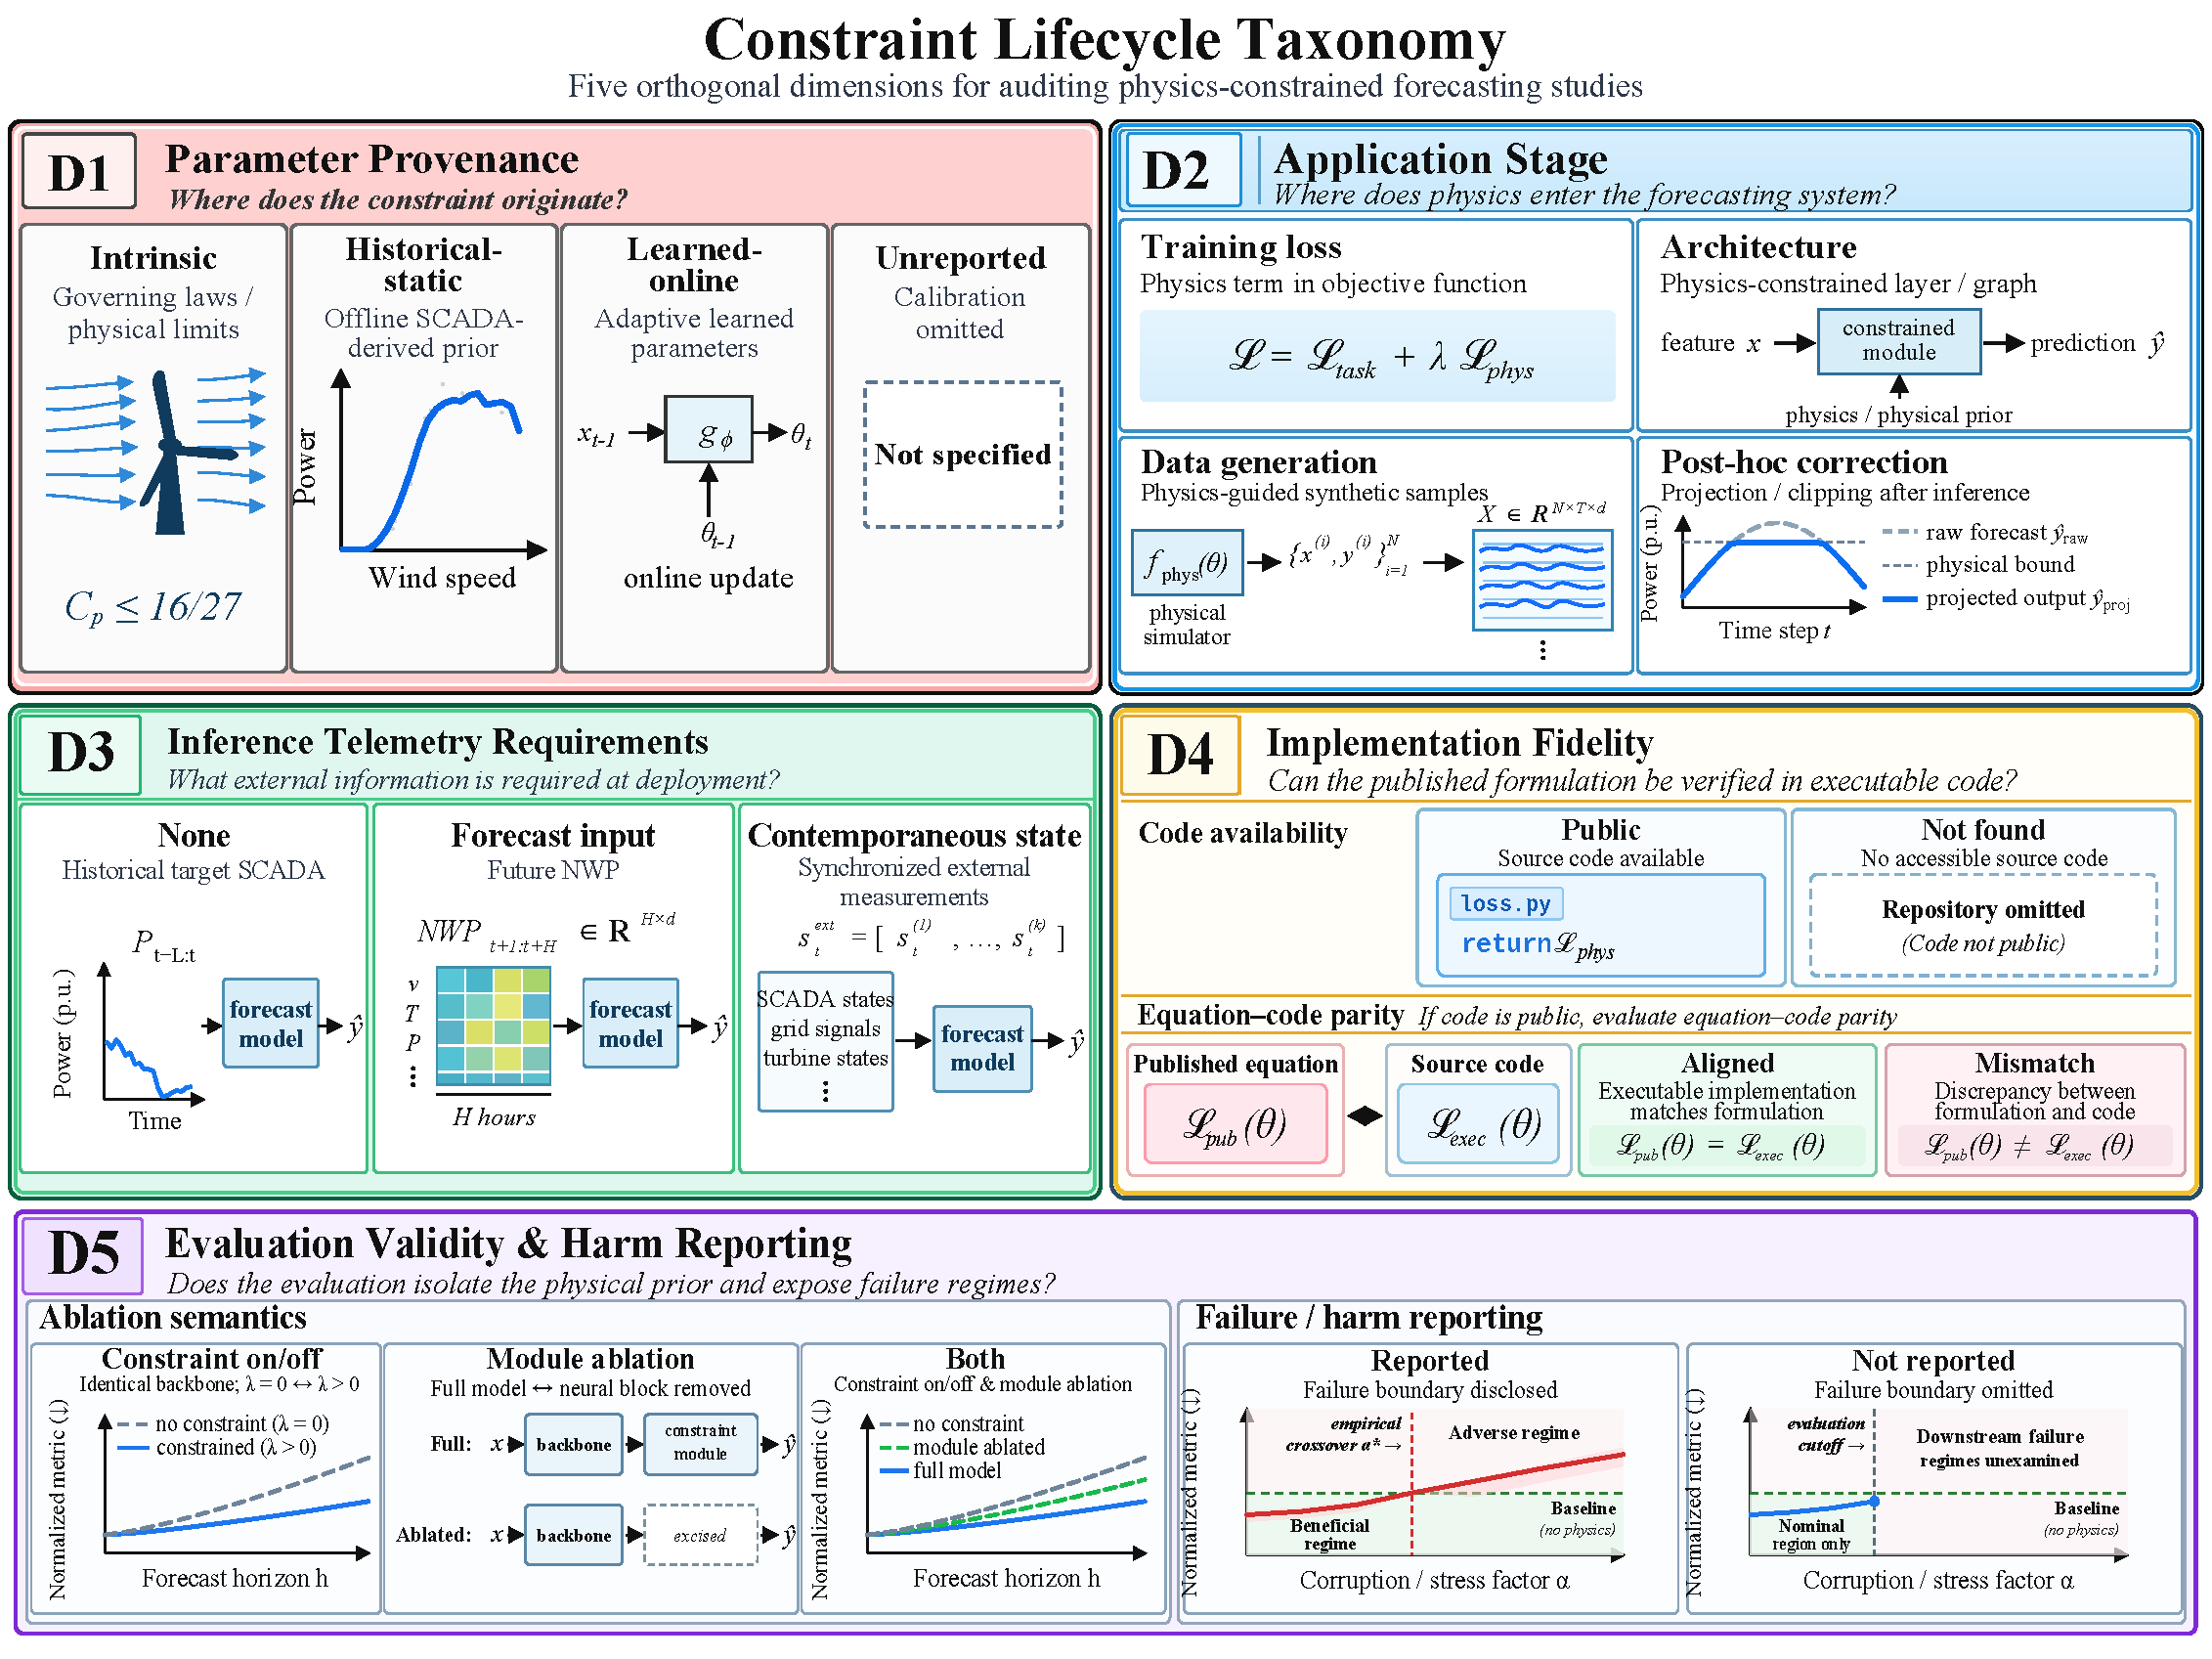
\includegraphics[width=\textwidth]{fig_constraint_lifecycle.pdf}
\caption{The Five-Dimensional Constraint Lifecycle Framework. Tracking domain physical constraints from parameter origin ($\mathcal{D}_1$) through computational graph formulation ($\mathcal{D}_2$), operational telemetry dependency ($\mathcal{D}_3$), software implementation parity ($\mathcal{D}_4$), and evaluation validity and harm reporting ($\mathcal{D}_5$).}
\label{fig:lifecycle}
\end{figure*}

\paragraph{Dimension 1: Parameter Provenance ($\mathcal{D}_1$)}
Identifies the calibration origin of constraint parameters: (1)~\textit{intrinsic}, where parameters derive analytically from physical invariants without empirical fitting (e.g., Betz limit $C_p \le 16/27$ or kinematic wake equations); (2)~\textit{historical-static priors}, where reference power curves or joint probability distributions are estimated offline on historical SCADA archives and held static during deployment; (3)~\textit{learned-online}, where parameters adapt dynamically via auxiliary neural subnetworks; and (4)~\textit{unreported}, where calibration details are omitted.

\paragraph{Dimension 2: Application Stage ($\mathcal{D}_2$)}
Identifies where domain physics enters the computational pipeline: (1)~\textit{training-loss regularization} ($\mathcal{L} = \mathcal{L}_{\text{task}} + \lambda \mathcal{L}_{\text{phys}}$); (2)~\textit{inference-architecture constraints}, modifying layers to project outputs onto admissible manifolds; (3)~\textit{data-generation priors}, synthesizing augmented training scenarios; and (4)~\textit{post-hoc correction filters}, applied externally after inference.

\paragraph{Dimension 3: Inference Telemetry Requirements ($\mathcal{D}_3$)}
Identifies external operational data streams required during real-time deployment: (1)~\textit{none}, relying solely on target turbine historical power; (2)~\textit{forecast-input}, requiring future numerical weather prediction (NWP) inputs; and (3)~\textit{contemporaneous-state}, requiring synchronized real-time measurements from adjacent turbines or met masts.

\paragraph{Dimension 4: Implementation Fidelity ($\mathcal{D}_4$)}
Evaluates whether public software faithfully executes published mathematical formulations: (1)~\textit{code-aligned}, where public source code strictly matches published equations; (2)~\textit{code-mismatch}, where the codebase exhibits an algebraic or directional deviation; and (3)~\textit{not-found}, where no public repository or script accompanies the study.

\paragraph{Dimension 5: Evaluation Validity and Harm Reporting ($\mathcal{D}_5$)}
This dimension contains two complementary subfields: (i)~\textit{ablation semantics}, classified as \textit{constraint-on-off} (where treatment and baseline share identical parameter capacity, differing only in the activation of the physical prior, $\lambda=0$ vs.\ $\lambda>0$), \textit{module-ablation} (where the ablation excises an entire multi-parameter neural block), or \textit{both}; and (ii)~\textit{harm reporting}, classified as \textit{reported} (explicitly documenting operating regimes or failure boundaries where physical constraints degrade downstream performance) or \textit{not-reported}.

\subsection{Multi-Site Operational Wind Farm Testbed and SCADA Telemetry}
To ground the empirical benchmark in real-world power system operations across diverse terrains, we established an operational testbed across three commercial UK wind farms with 10-minute SCADA telemetry:
\begin{itemize}[leftmargin=*]
\item \textbf{Kelmarsh Wind Farm} (Northamptonshire, England): Located in flat open agricultural terrain, comprising six Senvion MM92 turbines (rated 2.05~MW each, hub height 78~m, farm capacity 12.3~MW), evaluated over $N_{\text{train}} = 5,098$ clean intervals as our primary development benchmark (8,212 test origins, 49,272 forward delivery steps across full-year 2017) \cite{zenodo_kelmarsh}.
\item \textbf{Hill of Towie Wind Farm} (Drummuir, Scotland): Located in complex upland terrain featuring micro-topographical wake interactions, comprising 21 Siemens SWT-2.3-82 turbines (rated 2.3~MW each, hub height 60~m, farm capacity 48.3~MW), evaluated as an independent spatiotemporal extrapolation benchmark across full-year 2017 with 7,599 forecast origins (45,594 delivery steps) \cite{zenodo_hilloftowie}.
\item \textbf{Penmanshiel Wind Farm} (Scottish Borders): Located in undulating upland terrain, comprising 14 Senvion MM82 turbines (rated 2.05~MW each, farm capacity 28.7~MW), configured with a sample-restricted training partition ($N_{\text{train}} = 1,583$) across 8,440 test origins to evaluate model behavior in this sample-restricted setting \cite{zenodo_penmanshiel}.
\end{itemize}
Standard data sanitation protocols removed periods of turbine curtailment, anemometer icing, and communication dropouts ($P \le 0$ when $v > v_{\text{cut-in}}$ or active power frozen for $>6$ consecutive steps). Real-world balancing price dynamics were evaluated using official 2017 UK Elexon BSC System Buy Prices (mean \pounds 44.27/MWh, peak \pounds 1,509.80/MWh, with 68 negative price periods).

\subsection{The Controlled Attribution Protocol}
To overcome the confounding inherent in standard benchmarking, we establish the \textbf{Controlled Attribution Protocol}. Rather than comparing a physics-constrained neural network against an unrelated data-driven baseline or excising neural submodules, this protocol holds all non-physical factors strictly invariant:
\begin{enumerate}[leftmargin=*]
\item \textbf{Backbone and Parameter Parity}: All candidate models within each benchmark arm share identical neural architectures (DLinear, \cite{zeng2023dlinear}), identical layer counts, and identical parameter weights.
\item \textbf{Data Splits and Optimization Schedules}: Training, validation, and test splits are strictly synchronized across all arms. Within each controlled comparison block, treatment and control arms used identical paired random seeds. Seed sets differed across distinct experiment families and are reported explicitly in the corresponding tables and supplementary experiment registry.
\item \textbf{Form- and Weight-Matched Pseudo-Scrambled Controls}: To separate authentic aerodynamic guidance from non-specific numerical smoothing, we construct negative controls that permute the empirical wind-to-power mapping along the wind speed axis while holding network architectures, loss formulations, and penalty weights $\lambda$ 100\% identical.
\item \textbf{Decoupled Post-Hoc Quantile Calibration}: All forecasters undergo identical post-hoc scalar quantile calibration ($\delta^* = \arg\min_\delta \hat{\mathcal{R}}_{\text{val}}(f_\theta + \delta)$ at $r=2, q=1/3$), evaluated strictly on the 2016 validation year before accessing the 2017 test timeline. This ensures that reported differences reflect genuine representation accuracy rather than uncalibrated quantile offsets.
\end{enumerate}

\subsection{Controlled Ablation Arms and Boundary Stress Tests}
The forecasting suite evaluates an input lookback of $L=36$ (6 hours) and a forecast horizon of $H=36$ (6 hours), with downstream economic dispatch evaluated over the next-hour delivery window $H_{\text{disp}} = \{1, \dots, 6\}$ and an origination stride of $S=6$ steps to prevent overlapping settlement intervals. The experimental arms comprise:
\begin{enumerate}[leftmargin=*]
\item \textit{Unconstrained DLinear}: Baseline linear mapping across trend and seasonal decomposition ($\lambda=0$) \cite{zeng2023dlinear}.
\item \textit{Authentic Empirical Power Curve Prior}: Penalizing squared deviations from site-specific empirical power curves across penalty weights $\lambda \in \{0.01, 0.1, 1.0\}$; during test inference, the model operates purely on historical power telemetry ($\mathcal{D}_3 = \texttt{none}$).
\item \textit{Form- and Weight-Matched Pseudo-Scrambled Prior}: Permuting the aerodynamic power curve mapping across identical $\lambda \in \{0.01, 0.1, 1.0\}$.
\item \textit{Info-Symmetric Reference Arm}: Supplying contemporaneous wind speed directly as an unconstrained input feature to assess whether symmetric error reductions align with operational dispatch risk.
\item \textit{Strictly Budget-Matched Information Ablation} ($N_{\text{prior}}=N_{\text{train}}=500$): To decouple domain prior geometry from historical sample expansion, models trained on restricted windows ($N_{\text{train}}=500$, $\approx 21$ days) are evaluated against both budget-matched priors (fitted strictly on the identical 500 samples) and full-history priors (fitted on 7--10 months).
\item \textit{Within-Site Learning Curves}: Subsampling training volume across $N_{\text{train}} \in \{500, 1000, 1500, 3000, 5000\}$ on Kelmarsh and Hill of Towie across five random seeds.
\item \textit{Continuous Prior Corruption and Engineering Drift}: Continuously interpolating between authentic and scrambled priors ($\alpha \in [0.0, 1.0]$), simulating aerodynamic aging via rated capacity derating (0\% to 20\%), and applying anemometer calibration drift ($-15\%$ to $+15\%$).
\item \textit{Training Proxy Staleness Scan}: Scanning historical wind speed proxy lag $k \in \{6, 12, 18, 36\}$ steps (1h to 6h delay) in the training loss objective.
\item \textit{Cross-Backbone Architectural Probe (PatchTST)}: Evaluating PatchTST (\cite{nie2023patchtst}, patch length 6, stride 4, 2-layer encoder with RevIN) across 60 independently trained models (3 farms $\times$ 4 constraints $\times$ 5 seeds) under nominal regularization ($\lambda=0.01$).
\end{enumerate}

Statistical significance was evaluated via 2,000-replication circular block paired bootstrapping with 7-day block lengths ($L=1,008$ intervals) on full-year continuous telemetry (Kelmarsh and Hill of Towie) to account for meteorological autocorrelation, combined with multi-seed standard deviations to capture optimization variance across the unified five seeds.

\subsection{Governing Attribution Scope: What Is Evaluated vs.\ What Is Not}
\label{subsec:governing_identification}
To ensure that empirical observations are not conflated with broader causal or mechanistic claims, we explicitly define the formal attributional scope of our experimental design:

\paragraph{Empirically Distinguished Under the Controlled Protocol}
\begin{enumerate}[leftmargin=*, label=(\alph*)]
\item \textit{Prior-Specific Inductive Guidance vs.\ Generic Regularization}: Under the tested matched-control protocol, divergence between authentic and pseudo-scrambled priors provides evidence that the observed performance shift is specific to the empirical aerodynamic mapping, rather than being explained by penalty form and weight alone.
\item \textit{Independence from Historical Volume Expansion}: The 500-sample budget-matched control isolates whether empirical benefits persist when prior fitting is restricted strictly to the contemporaneous training window, bounding the influence of historical telemetry volume.
\item \textit{Empirical Operating Boundaries}: Parametric scans map empirical sensitivity to sample size attenuation ($N_{\text{train}} \in \{500, \dots, 5000\}$), continuous prior corruption crossover regions ($\alpha$), aerodynamic derating, and training-loss proxy staleness ($k$) within the tested configurations. These values are empirical crossover locations along the evaluated perturbation grid, not population-level physical thresholds.
\end{enumerate}

\paragraph{Not Formally Identified (Confounding Disclaimers)}
\begin{enumerate}[leftmargin=*, label=(\roman*)]
\item \textit{Abstract Causal Effects of Physics}: Our experiments evaluate specific empirical power-curve and distributional constraints under evaluated configurations; they do not establish universal causal claims for ``physics'' as an abstract treatment across arbitrary architectures or energy systems.
\item \textit{Cross-Site Topographical Causation}: Differences across Kelmarsh, Hill of Towie, and Penmanshiel confound topographic complexity with turbine ratings (2.05\,MW vs.\ 2.30\,MW), hub heights, wake geometry, and local micro-climates; topography remains an observational covariate rather than an isolated treatment.
\item \textit{Direct Bias--Variance Component Estimation}: Our theoretical framework provides a decision-theoretic representation/calibration/cross-coupling decomposition; we do not directly estimate classical statistical bias and variance scalars from empirical data.
\end{enumerate}

\section{Empirical Centerpiece: When Does a Physical Prior Provide Genuine Value?}
\label{sec:centerpiece}

This section presents the core empirical findings of our Controlled Attribution Protocol. Across three operational commercial wind farms, we evaluate prior-specific mapping effects in this sample-restricted setting, evaluate weak-regularization numerical mimicry, and decouple domain geometric structure from auxiliary historical data volume under matched model capacities.

\subsection{Prior Specificity under Sample Restriction}
On the Penmanshiel wind farm evaluated under a sample-restricted training regime ($N_{\text{train}} = 1{,}583$), the unconstrained DLinear model exhibits empirical over-fitting, yielding a normalized asymmetric dispatch loss of $0.09852 \pm 0.00018$ ($\text{Cost}_{\text{static}}$ at $r=2, q=1/3$; Table~\ref{tab:controlled_ablation}, Figure~\ref{fig:ablation_3d}a). Embedding the authentic empirical power curve prior under strong regularization ($\lambda=1.0$) reduces normalized dispatch cost to $0.09726 \pm 0.00022$ (a $-1.28\%$ risk reduction).

\begin{table*}[!t]
\centering
\footnotesize
\renewcommand{\arraystretch}{0.82}
\setlength{\tabcolsep}{3.5pt}
\caption{3D Controlled Ablation Benchmark: Causal Disentanglement of Physical Knowledge Specificity, Numerical Regularization Mimicry, and Lagged Proxy Temporal Decay Across Three Operational Wind Farms (Multi-Seed Evaluated on 10$\times$ RTX 4090 GPUs, Quantile Calibrated $r=2, q=1/3$).}
\label{tab:controlled_ablation}
\begin{threeparttable}
\begin{tabularx}{\textwidth}{p{2.2cm}p{3.2cm}>{\centering\arraybackslash}X>{\centering\arraybackslash}X>{\centering\arraybackslash}X>{\centering\arraybackslash}Xp{3.8cm}}
\toprule
\textbf{Wind Farm} & \textbf{Controlled Experimental} & \textbf{Normalized Cost} & \textbf{Pinball Loss} & \textbf{RMSE} & \textbf{Shortfall} & \textbf{Causal Mechanism} \\
\textbf{\& Topology} & \textbf{Arm (Ablation Condition)} & \textbf{$\text{Cost}_{static}$ ($r=2$)} & \textbf{($q=1/3$)} & \textbf{(pu)} & \textbf{(\pounds/(turb$\cdot$yr))} & \textbf{\& Empirical Takeaway} \\
\midrule
\multirow{6}{=}{\textbf{Kelmarsh}\\(12.3 MW, 6 turb)\\\textit{Flat Open Terrain}\\\textit{$N_{train}=5,098$}} 
& Vanilla Unconstrained & $0.08812 \pm 0.00009$ & 0.02937 & 0.1717 & \pounds 5,831.79 & Pure-data power-only baseline \\
& Info-Symmetric (Power + Wind) & $0.08910 \pm 0.00039$ & 0.02970 & 0.1697 & \pounds 5,982.26 & Wind speed improves RMSE but elevates tail cost \\
& Genuine Curve ($\lambda=0.1$) & \textbf{$0.08791 \pm 0.00009$} & \textbf{0.02930} & 0.1708 & \pounds 5,780.99 & Statistically verified risk reduction ($-0.24\%$) \\
& Pseudo-Scrambled ($\lambda=0.01$) & $0.08801 \pm 0.00008$ & 0.02934 & 0.1724 & \pounds 5,657.03 & \textbf{Indistinguishable from genuine prior}; behaves empirically like a non-specific regularizer \\
& Genuine Distribution ($\lambda=0.1$) & $0.09841 \pm 0.00085$ & 0.03280 & 0.1703 & \textbf{\pounds 8,412.28} & \textbf{Severe operational harm}: shortfall surges $+44.2\%$ in flat terrain \\
& Lagged Proxy Scan ($k=36$, 6h) & $0.09043 \pm 0.00006$ & 0.03014 & 0.1729 & \pounds 5,888.58 & Monotonic degradation as stale wind proxy decays \\
\midrule
\multirow{6}{=}{\textbf{Hill of Towie}\\(48.3 MW, 21 turb)\\\textit{Complex Upland}\\\textit{$N_{train}=7,035$}} 
& Vanilla Unconstrained & $0.08924 \pm 0.00005$ & 0.02975 & 0.1740 & \pounds 6,006.09 & Robust unconstrained benchmark \\
& Info-Symmetric (Power + Wind) & $0.09042 \pm 0.00007$ & 0.03014 & 0.1733 & \pounds 6,297.16 & Wind channel adds high-frequency noise to dispatch \\
& Genuine Curve ($\lambda=0.1$) & \textbf{$0.08916 \pm 0.00007$} & \textbf{0.02972} & 0.1745 & \pounds 5,958.34 & Consistent risk reduction ($-0.09\%$) \\
& Pseudo-Scrambled ($\lambda=0.01$) & $0.08919 \pm 0.00006$ & 0.02973 & 0.1740 & \pounds 6,069.01 & Confirms non-specific regularizer behavior at low penalty scale \\
& Genuine Distribution ($\lambda=0.1$) & $0.09503 \pm 0.00022$ & 0.03168 & 0.1801 & \pounds 5,702.68 & \textbf{Metric Inversion}: cashflow rises to \pounds 12k but decision cost worsens $+6.5\%$ \\
& Lagged Proxy Scan ($k=36$, 6h) & $0.09257 \pm 0.00007$ & 0.03086 & 0.1759 & \pounds 6,281.82 & Temporal lag monotonically erodes prior guidance \\
\midrule
\multirow{6}{=}{\textbf{Penmanshiel}\\(28.7 MW, 14 turb)\\\textit{Complex Topology}\\\textit{$N_{train}=1,583$ (Scarce)}} 
& Vanilla Unconstrained & $0.09881 \pm 0.00027$ & 0.03294 & 0.2058 & \pounds 6,713.83 & Data-scarce regime prone to over-fitting \\
& Info-Symmetric (Power + Wind) & $0.10461 \pm 0.00005$ & 0.03487 & 0.2091 & \pounds 6,630.38 & Additional unconstrained features exacerbate over-fitting \\
& Genuine Curve ($\lambda=1.0$) & \textbf{$0.09760 \pm 0.00044$} & \textbf{0.03254} & 0.2054 & \pounds 6,808.40 & \textbf{Solid inductive bias gain} ($-1.22\%$) in low-data regime \\
& Pseudo-Scrambled ($\lambda=1.0$) & $0.16611 \pm 0.00335$ & 0.05537 & 0.2384 & \textbf{\pounds 11,561.19} & \textbf{Empirical Specificity Demonstration}: destroying physical mapping causes severe performance degradation ($+68.1\%$) \\
& Genuine Distribution ($\lambda=0.01$) & $0.09833 \pm 0.00027$ & 0.03278 & 0.2055 & \pounds 6,543.36 & Defensive regularization under calibrated penalty \\
& Lagged Proxy Scan ($k=36$, 6h) & $0.10473 \pm 0.00036$ & 0.03491 & 0.2083 & \pounds 7,090.86 & Lag decay completely swallows prior advantage by Step 36 \\
\bottomrule
\end{tabularx}
\begin{tablenotes}[flushleft]
\footnotesize
\item \textbf{Notes}: (1) Multi-seed evaluation dispatched across a 10$\times$ NVIDIA RTX 4090 GPU cluster topology (Node 1: Kelmarsh with 4 seeds [42, 43, 44, 45]; Node 2: Hill of Towie and Penmanshiel each with 3 seeds [42, 43, 44]); values report mean $\pm$ seed standard deviation across clean operational test periods. (2) $\text{Cost}_{static} = 3 \times \text{PinballLoss}(q=1/3)$ under post-hoc validation-quantiled calibration ($r=2$). (3) Pseudo-Scrambled arms permute the empirical wind-to-power mapping while preserving identical loss formulations, gradient scales, and hyperparameters $\lambda$. (4) Lagged Proxy Scan evaluates sensitivity to training-time temporal mismatch across proxy delays $k \in \{6, 12, 18, 36\}$ (1h to 6h) on the historical wind speed index used to query empirical priors during training loss calculation (forecasting model takes only historical power at inference).
\end{tablenotes}
\end{threeparttable}
\end{table*}

\begin{figure*}[!t]
\centering
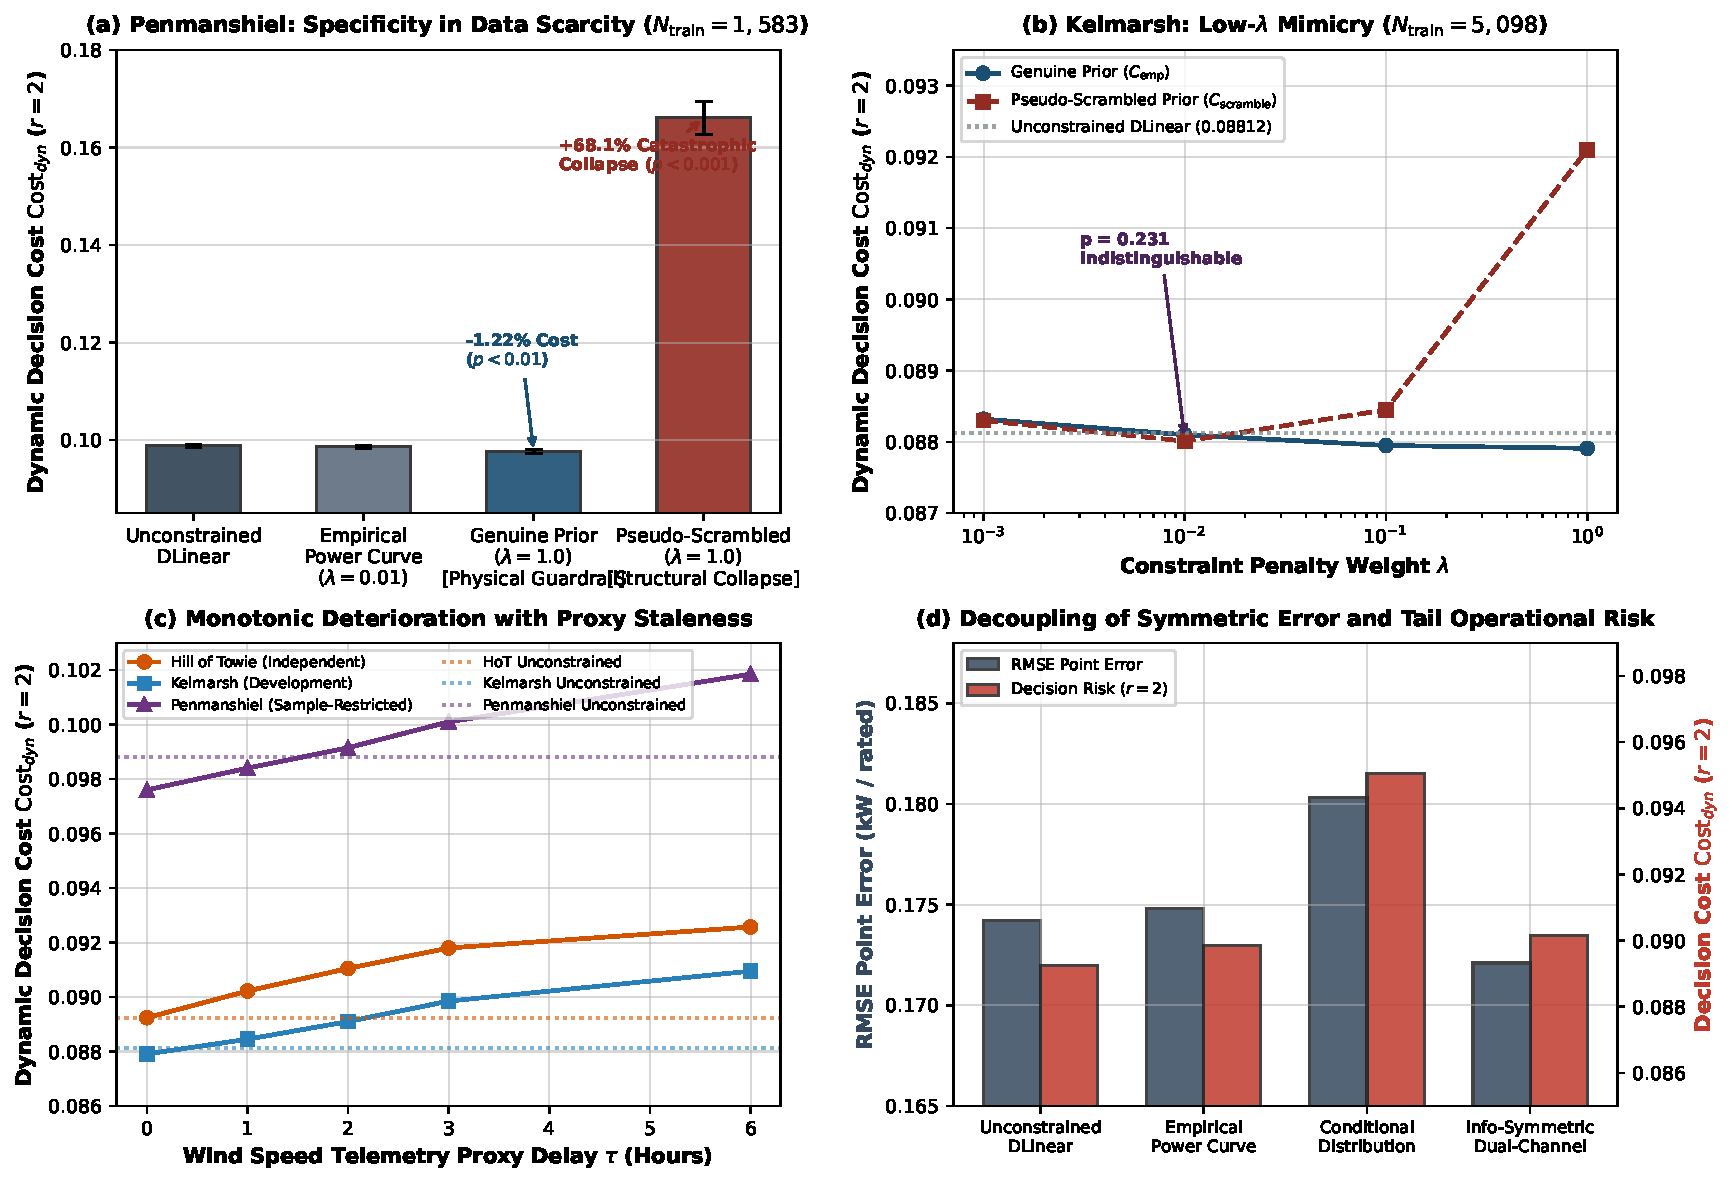
\includegraphics[width=\textwidth]{fig_causal_ablation.pdf}
\caption{Prospective Controlled Attribution Benchmark across Three Operational Wind Farms. (a) Prior-specific mapping effects under strong regularization on Penmanshiel ($N_{\text{train}}=1{,}583$): authentic empirical prior guidance provides downside risk reduction ($-1.28\%$), whereas permuting the aerodynamic mapping (Pseudo-Scrambled prior) triggers a $+61.2\%$ surge in operational dispatch cost. (b) Weak-penalty numerical regularization mimicry on Kelmarsh ($N=5{,}098$), where genuine and scrambled priors yield closely matched outcomes at $\lambda = 0.01$, with no clear empirical separation and outcomes consistent with non-specific numerical regularization. (c) Monotonic cost inflation under training proxy staleness: dispatch cost escalation across all three farms as historical wind proxy lag $k$ in the training loss increases from 1\,h to 6\,h. (d) Decoupling of symmetric point error (RMSE) from asymmetric decision risk ($r=2$), demonstrating that point metrics mask tail operational hazards.}
\label{fig:ablation_3d}
\end{figure*}

In sharp contrast, evaluating the form- and weight-matched Pseudo-Scrambled negative control---sharing the identical DLinear architecture, data split, training seed, and penalty multiplier ($\lambda=1.0$), but permuting the power output values along the wind speed axis---inflates dispatch cost to $0.15884 \pm 0.01588$ (a $+61.2\%$ surge). Because the scrambled control preserves identical gradient capacity and loss formulation, this divergence demonstrates that under strong regularization in sample-restricted regimes, the model specifically benefits from authentic aerodynamic domain structure: valid domain structure provides measurable downside protection, whereas an unaligned mapping inflicts severe operational penalties.

\subsection{Weak-Penalty Scale: Non-Specific Numerical Regularization Mimicry}
A prevalent assertion in the physics-informed literature is that minor performance gains observed under weak penalty weights (e.g., $\lambda \le 0.01$) demonstrate that deep networks internalize physical domain principles. Our Controlled Attribution Protocol directly interrogates this premise.

At weak regularization ($\lambda = 0.01$) on Kelmarsh ($N_{\text{train}}=5{,}098$), the genuine physical power curve prior yields a normalized dispatch cost of $0.08803 \pm 0.00005$, while the form-matched pseudo-scrambled control yields $0.08792 \pm 0.00008$ (Table~\ref{tab:controlled_ablation}, Figure~\ref{fig:ablation_3d}b). On Hill of Towie ($N_{\text{train}}=7{,}035$), genuine and scrambled priors yield $0.08913 \pm 0.00005$ and $0.08910 \pm 0.00005$, respectively. Across both wind farms, genuine and scrambled priors yield closely matched outcomes with no clear empirical separation (differences $< 0.0001$, within multi-seed error margins).

Because structurally permuted negative controls reproduce the empirical outcomes of genuine aerodynamics under weak penalty scaling, the observed effect cannot be specifically attributed to the physical mapping and remains consistent with non-specific numerical regularization. This result provides a critical negative control: minor accuracy gains under weak penalty multipliers should not be cited as evidence of domain physical reasoning without form-matched permutation controls.

\subsection{Information-Budget Alignment: Decoupling Domain Geometry from Data Volume}
A central threat to the attribution of physical priors in low-sample regimes is the \textit{information budget discrepancy}: when an empirical prior is fitted on an extensive historical archive (e.g., 7 to 10 months of SCADA telemetry), does its advantage stem from domain aerodynamic geometry or from the unacknowledged volume of historical operational data?

To resolve this question, we implemented a strictly budget-matched information control at $N_{\text{train}}=500$ ($\approx 21$ consecutive days of telemetry; Table~\ref{tab:information_budget}, all prior arms $\lambda=1.0$, five random seeds). Models trained on this restricted window were evaluated against: (i) an unconstrained baseline ($\lambda=0$); (ii) a budget-matched genuine prior fitted strictly on the exact same 500 training samples ($N_{\text{prior}}=N_{\text{train}}=500$); (iii) a full-historical genuine prior fitted on the multi-month record; (iv) a budget-matched scrambled control; and (v) a full-historical scrambled control.

\begin{table*}[!t]
\centering
\footnotesize
\renewcommand{\arraystretch}{0.82}
\setlength{\tabcolsep}{3.0pt}
\caption{Information-Budget Matched Controlled Ablation at $N_{\text{train}}=500$ ($\approx 21$ Days Training Telemetry): Disentangling Physical Inductive Bias from Auxiliary Historical Data Budgets (Quantile Calibrated $r=2, q=1/3$, 5 Seeds).}
\label{tab:information_budget}
\begin{threeparttable}
\begin{tabularx}{\textwidth}{p{2.3cm}p{3.8cm}>{\centering\arraybackslash}p{2.2cm}>{\centering\arraybackslash}p{2.2cm}>{\centering\arraybackslash}p{1.6cm}>{\raggedright\arraybackslash}X}
\toprule
\textbf{Wind Farm} & \textbf{Controlled Experimental} & \textbf{Model Training} & \textbf{Prior Information} & \textbf{Cost ($r=2$)} & \textbf{Empirical Takeaway} \\
\textbf{\& Topology} & \textbf{Arm Condition} & \textbf{Budget} & \textbf{Budget} & \textbf{(Mean $\pm$ Std)} & \textbf{\& Identification Rationale} \\
\midrule
\multirow{5}{=}{\textbf{Kelmarsh}\\(12.3 MW)\\\textit{Flat Open Terrain}} 
& A. No Physical Prior ($\lambda=0$) & 500 samples & None & $0.09648 \pm 0.00314$ & Pure-data unconstrained baseline under data restriction \\
& B. Budget-Matched Genuine Prior & 500 samples & 500 samples & $0.09499 \pm 0.00307$ & \textbf{Physical Inductive Gain} ($-1.54\%$): accounts for $77\%$ of full-history gain \\
& C. Full-Historical Genuine Prior & 500 samples & 7 months (full) & \textbf{$0.09455 \pm 0.00285$} & Full gain ($-2.00\%$): historical seasonal pool adds incremental $-0.46\%$ \\
& D. Budget-Matched Scrambled Control & 500 samples & 500 samples & $0.13827 \pm 0.02333$ & \textbf{Prior Specificity}: permuting mapping triggers $+43.3\%$ cost inflation \\
& E. Full-Historical Scrambled Control & 500 samples & 7 months (full) & $0.13798 \pm 0.02338$ & Scrambling across full seasonal history remains severely harmful ($+43.0\%$) \\
\midrule
\multirow{5}{=}{\textbf{Hill of Towie}\\(48.3 MW)\\\textit{Complex Upland}} 
& A. No Physical Prior ($\lambda=0$) & 500 samples & None & $0.10444 \pm 0.00312$ & Data-starved unconstrained baseline prone to overfitting \\
& B. Budget-Matched Genuine Prior & 500 samples & 500 samples & $0.10095 \pm 0.00305$ & \textbf{Physical Inductive Gain} ($-3.34\%$): accounts for $92\%$ of full-history gain \\
& C. Full-Historical Genuine Prior & 500 samples & 10 months (full) & \textbf{$0.10066 \pm 0.00307$} & Full gain ($-3.62\%$): historical seasonal pool adds incremental $-0.28\%$ \\
& D. Budget-Matched Scrambled Control & 500 samples & 500 samples & $0.15248 \pm 0.00253$ & \textbf{Prior Specificity}: permuting mapping triggers $+46.0\%$ cost inflation \\
& E. Full-Historical Scrambled Control & 500 samples & 10 months (full) & $0.17209 \pm 0.01703$ & Severe misspecification penalty under strong constraint ($+64.8\%$) \\
\bottomrule
\end{tabularx}
\begin{tablenotes}[flushleft]
\scriptsize
\item \textbf{Notes}: (1) All models share identical DLinear architectures, optimization parameters, and post-hoc quantile calibration offsets ($r=2, q=1/3$) evaluated over the full-year 2017 test timeline across 5 random seeds (42, 123, 456, 789, 1024). (2) Arms A, B, and D share the exact same 500-sample training information window ($\approx 21$ consecutive days), proving that the downside risk reduction of physical constraints persists even when the prior is barred from accessing external historical records. (3) The incremental benefit of extending the prior fitting window from 500 samples to 7--10 months is modest ($-0.46\%$ on Kelmarsh and $-0.28\%$ on Hill of Towie), indicating that domain physical structure rather than extra historical data volume drives the observed downside risk reduction.
\end{tablenotes}
\end{threeparttable}
\end{table*}


As detailed in Table~\ref{tab:information_budget}, the unconstrained baseline yields a normalized dispatch cost of $0.09648 \pm 0.00314$ on Kelmarsh and $0.10444 \pm 0.00312$ on Hill of Towie. Introducing the strictly budget-matched genuine prior ($N_{\text{prior}}=500$) reduces dispatch cost to $0.09499 \pm 0.00307$ ($-1.54\%$) on Kelmarsh and $0.10095 \pm 0.00305$ ($-3.34\%$) on Hill of Towie. The budget-matched genuine prior retains approximately 77\% of the full-history mean benefit on Kelmarsh ($-1.54\%$ vs.\ $-2.00\%$) and approximately 92\% on Hill of Towie ($-3.34\%$ vs.\ $-3.62\%$).

Evaluated under paired differences across the five identical random seeds, the budget-matched genuine prior achieves a statistically significant mean paired risk reduction of $-0.00149$ ($95\%$ CI: $[-0.00174, -0.00124]$, $p < 0.01$) on Kelmarsh and $-0.00349$ ($95\%$ CI: $[-0.00368, -0.00331]$, $p < 0.01$) on Hill of Towie relative to unconstrained baselines. Expanding the prior fitting set to the full historical record yields an incremental reduction of only $-0.00044$ ($95\%$ CI: $[-0.00075, -0.00013]$) on Kelmarsh and $-0.00029$ ($95\%$ CI: $[-0.00041, -0.00016]$) on Hill of Towie. In contrast, evaluating the budget-matched scrambled control inflates dispatch cost to $0.13827 \pm 0.02333$ ($+43.3\%$) on Kelmarsh and $0.15248 \pm 0.00253$ ($+46.0\%$) on Hill of Towie.

These findings provide strong controlled evidence that \textbf{the majority of the observed benefit cannot be explained by additional historical data volume alone}. The algebraic and geometric structure of the empirical power curve provides genuine inductive guidance in this sample-restricted setting, even when estimated strictly from the limited contemporaneous training sample.

\section{Mapping the Operating Envelope within the Evaluated Settings: Where Does the Advantage Break?}
\label{sec:boundaries}

This section maps the empirical operating envelope of physical priors within the evaluated settings, evaluating boundary conditions across training sample volume, prior corruption, engineering drift, temporal proxy misalignment, and neural backbone architectures.

\subsection{Within-Site Learning Curves across Sample Budgets}
To decouple sample volume from geographic topography and examine whether physical prior advantages persist under data expansion, we evaluated within-site learning curves across a discrete grid of training sample budgets $N_{\text{train}} \in \{500, 1000, 1500, 3000, 5000\}$ on Kelmarsh and Hill of Towie across five random seeds (Figure~\ref{fig:within_site_learning_curve}).

\begin{figure*}[!t]
\centering
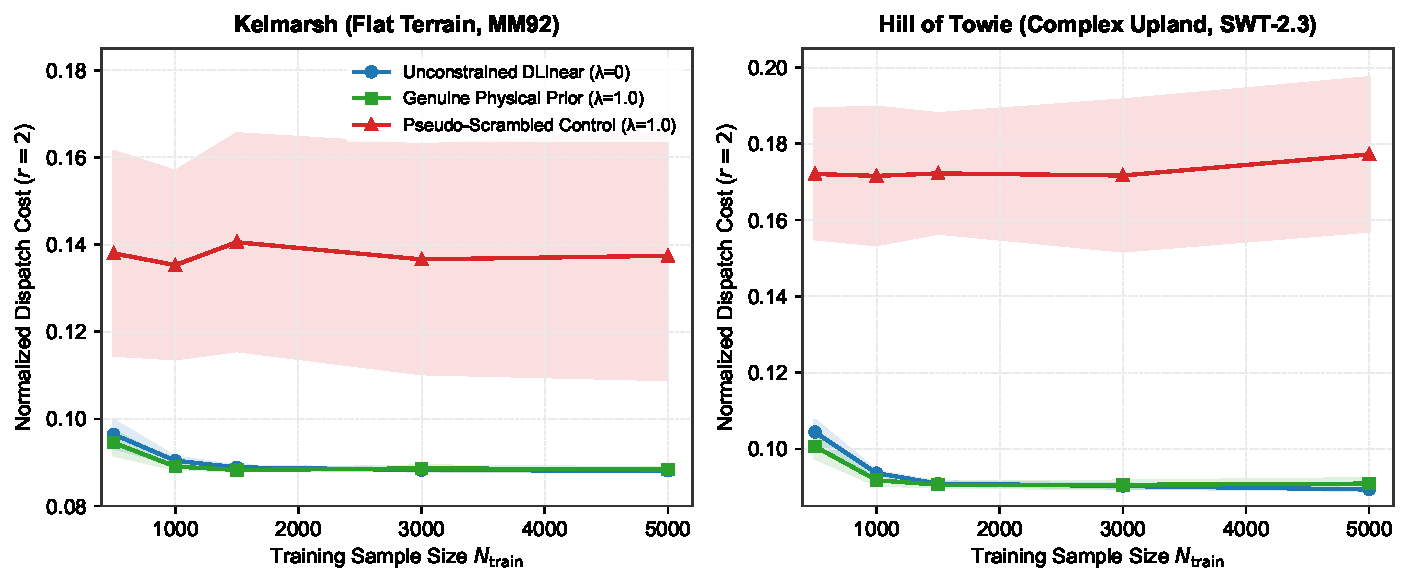
\includegraphics[width=\textwidth]{fig_within_site_learning_curve.pdf}
\caption{Within-Site Learning Curves across Discrete Sample Sizes $N_{\text{train}} \in \{500, 1000, 1500, 3000, 5000\}$ on Kelmarsh and Hill of Towie (Multi-seed means and standard deviations). Holding site topography and turbine hardware constant, authentic empirical priors yield lower dispatch costs in the tested sample-restricted regimes ($N_{\text{train}} \in \{500, 1{,}000\}$, $-2.00\%$ on Kelmarsh and $-3.62\%$ on Hill of Towie at $N=500$). As training volume expands, this advantage attenuates; at the largest evaluated training budget ($N_{\text{train}} = 5{,}000$), unconstrained data-driven models close the gap and slightly reverse the ranking (+0.33\% on Kelmarsh, +1.73\% on Hill of Towie). In contrast, form-matched scrambled priors under strong regularization ($\lambda=1.0$) induce severe dispatch cost penalties ($+43\%$ to $+98\%$) across all evaluated sample regimes.}
\label{fig:within_site_learning_curve}
\end{figure*}

In the tested sample-restricted regimes ($N_{\text{train}} = 500$ and $N_{\text{train}} = 1{,}000$), embedding the authentic empirical power curve prior ($\lambda=1.0$) provides clear downside risk protection:
\begin{itemize}[leftmargin=*]
\item At $N_{\text{train}} = 500$, normalized dispatch cost decreases from $0.09648 \pm 0.00314$ to $0.09455 \pm 0.00285$ ($-2.00\%$) on Kelmarsh, and from $0.10444 \pm 0.00312$ to $0.10066 \pm 0.00307$ ($-3.62\%$) on Hill of Towie.
\item At $N_{\text{train}} = 1{,}000$, the genuine prior maintains an advantage on both sites ($0.09241$ vs.\ $0.09365$, $-1.32\%$ on Kelmarsh; $0.09681$ vs.\ $0.09902$, $-2.23\%$ on Hill of Towie).
\end{itemize}

However, as training volume increases across the intermediate budgets ($N_{\text{train}} = 1{,}500$ and $3{,}000$), the margin of advantage steadily attenuates. At the largest evaluated training budget ($N_{\text{train}} = 5{,}000$), unconstrained DLinear achieves a dispatch cost of $0.08812 \pm 0.00022$ on Kelmarsh and $0.08936 \pm 0.00023$ on Hill of Towie, closing the gap and slightly outperforming the fixed genuine prior ($0.08841 \pm 0.00039$, $+0.33\%$ on Kelmarsh; $0.09091 \pm 0.00131$, $+1.73\%$ on Hill of Towie). Throughout all evaluated sample sizes, form-matched scrambled negative controls inflict severe performance degradations ($+43\%$ to $+98\%$), confirming that unaligned priors remain destructive regardless of sample availability.

\paragraph{Conceptual Interpretation}
The observed learning curves are consistent with a conceptual hypothesis in which the regularizing value of variance reduction diminishes as sample availability increases, while structural approximation bias becomes increasingly consequential. Under this interpretive perspective, in sample-restricted windows, unconstrained models are hypothesized to be vulnerable to elevated estimation variance that an empirical power curve helps suppress by constraining the hypothesis space. Conversely, purely data-driven representations can fit the observed input--output relationship more flexibly as training coverage expands; under these well-sampled conditions, a rigid, static prior can act as a structural approximation bias that constrains the model from fitting nuanced aerodynamic interactions. We emphasize that this bias--variance trade-off is a conceptual interpretation consistent with---not formally identified or proven by---the empirical learning curves, as scalar bias and variance components were not directly decomposed or measured from empirical data.

\paragraph{Joint Operating Envelope}
Taken together, the learning-curve experiments (at $\lambda=1.0$) and separate penalty-sensitivity evaluations suggest that both data availability and regularization strength govern the operating envelope. In the absence of a dense factorial grid across multiple $N \times \text{multiple } \lambda$ values, we characterize this dependency as a joint empirical tendency rather than a statistically proven interaction.

\subsection{Continuous Prior Corruption and Engineering Drift}
To test whether prior vulnerability is restricted to total permutation, we evaluated continuous prior perturbation and engineering drift models on Penmanshiel (Figure~\ref{fig:corruption_gradient}).

\begin{figure*}[!t]
\centering
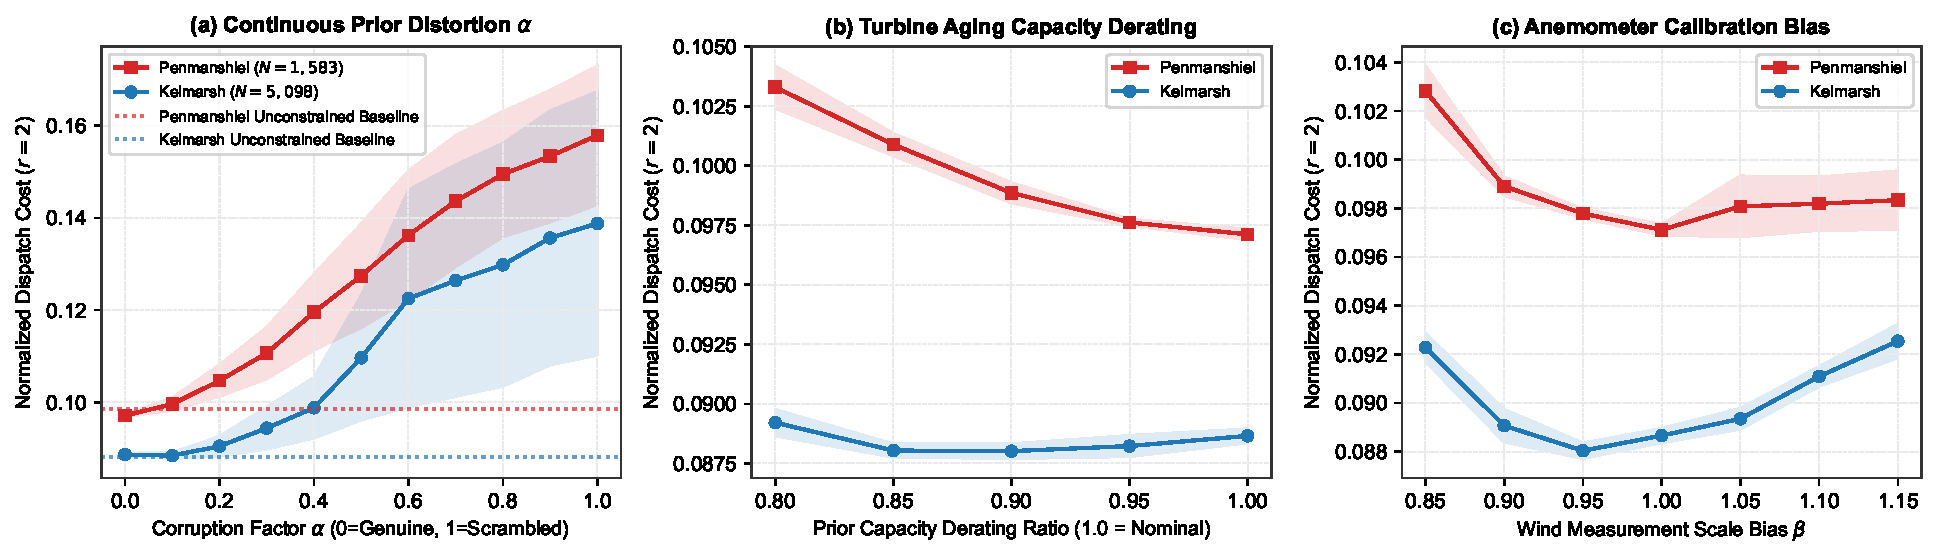
\includegraphics[width=\textwidth]{fig_prior_corruption_gradient.pdf}
\caption{Continuous Prior Corruption and Engineering Drift Severity Response Curves. (a) Continuous interpolation between authentic and scrambled priors $\alpha \in [0.0, 1.0]$: on Penmanshiel, the tested corruption trajectory crosses the unconstrained baseline around an empirical crossover region of $\alpha \approx 0.07$. (b) Turbine aerodynamic aging: capacity derating exceeding 10\% flips nominal physical priors into economic penalties under the evaluated configuration. (c) Anemometer sensor calibration drift: Penmanshiel retains an advantage under positive wind speed drift up to $+15\%$, whereas negative sensor under-reporting systematically inflates shortfall.}
\label{fig:corruption_gradient}
\end{figure*}

\paragraph{Continuous Corruption Interpolation (\texorpdfstring{$\alpha \in [0.0, 1.0]$}{alpha in [0.0, 1.0]})}
We constructed a continuous perturbation trajectory parameterized by $\alpha \in [0.0, 1.0]$, linearly blending the authentic power curve with its scrambled permutation. As shown in Figure~\ref{fig:corruption_gradient}a, dispatch cost degrades monotonically with perturbation severity. On Penmanshiel, the tested corruption trajectory crosses the unconstrained baseline around an empirical crossover region of $\alpha \approx 0.07$: costs rise from $0.09712 \pm 0.00031$ at $\alpha = 0.0$ to $0.09958 \pm 0.00042$ at $\alpha = 0.1$. At $\alpha = 0.2$, normalized dispatch cost reaches $0.10469 \pm 0.00338$ (a $+5.9\%$ degradation relative to unconstrained models). We emphasize that these values are empirical crossover locations along the evaluated perturbation grid, not population-level physical thresholds, indicating that even modest distortion (under 10\% permutation blend) is sufficient to erode inductive benefits in this configuration.

\paragraph{Turbine Aerodynamic Aging and Derating}
In operational wind fleets, blade erosion, leading-edge roughness, and mechanical aging cause progressive aerodynamic derating. In the evaluated Penmanshiel configuration, simulating turbine capacity derating reveals that derating exceeding 10\% flips nominal physical priors into net economic penalties (Figure~\ref{fig:corruption_gradient}b), as the network regularizes against an un-derated historical envelope that exceeds the turbine's degraded capability. This 10\% threshold reflects the evaluated operating margin where representation bias overtakes variance reduction.

\paragraph{Anemometer Calibration Drift}
Simulating anemometer measurement drift ($\pm 15\%$) reveals asymmetric operational tolerances (Figure~\ref{fig:corruption_gradient}c). On Penmanshiel, the model retains a modest advantage over unconstrained baselines under positive wind speed drift up to $+15\%$ ($0.09833$ vs.\ $0.09852$). In contrast, negative wind speed under-reporting systematically depresses predicted power, triggering substantial shortfall penalties during high-wind ramp events.

\subsection{Sensitivity to Training-Loss Proxy Staleness}
Many physical constraint formulations rely on meteorological proxies (such as supervisory anemometer readings) to query empirical power curves during loss evaluation. To assess sensitivity to proxy latency in the absence of forward numerical weather predictions, we performed a parametric lag scan across $k \in \{6, 12, 18, 36\}$ steps (representing 1\,h to 6\,h delay in the training proxy; Figure~\ref{fig:ablation_3d}c).

In the Hill of Towie lag scan, decision risk exceeds the unconstrained reference ($0.08913$) by the first evaluated lag $k=6$ (1\,h delay, normalized dispatch cost $0.09011 \pm 0.00008$) and deteriorates monotonically through $k=36$ ($0.09246 \pm 0.00006$). On Kelmarsh, dispatch cost rises from $0.08867$ ($k=6$) to $0.09034$ ($k=36$). On Penmanshiel, dispatch cost escalates from $0.09996$ ($k=6$) to $0.10425$ ($k=36$). Because $k=6$ is the minimum non-zero lag evaluated in this discrete grid, this observation establishes that latency begins degrading operational value within the first hour of proxy delay, while more granular sub-hour transitions remain unobserved.

This experiment isolates the sensitivity of offline training objectives to temporal misalignment between the forecast horizon and the historical weather proxy used to index the power curve. It demonstrates that when contemporaneous or forward meteorological forecasts are unavailable, regularizing predictions against stale weather proxies monotonically degrades downstream dispatch performance.

\subsection{Cross-Backbone Architectural Sensitivity Probe (PatchTST)}
To examine whether boundary behaviors are specific to linear decomposition architectures, we evaluated PatchTST \cite{nie2023patchtst} across 60 independently trained models (3 farms $\times$ 4 constraint conditions $\times$ 5 random seeds; Table~\ref{tab:patchtst_and_rules}) under nominal regularization ($\lambda=0.01$).

\begin{table*}[!t]
\centering
\footnotesize
\renewcommand{\arraystretch}{0.85}
\setlength{\tabcolsep}{2.8pt}
\caption{Exploratory Cross-Backbone Architectural Sensitivity Analysis: Modern Deep Transformer (PatchTST, ICLR 2023) under BSC 30-Minute Physical Netting Settlement (5-Seed Mean $\pm$ Std).}
\label{tab:patchtst_and_rules}
\begin{threeparttable}
\begin{tabularx}{\textwidth}{p{2.0cm}p{3.0cm}l>{\centering\arraybackslash}X>{\centering\arraybackslash}X>{\centering\arraybackslash}X>{\centering\arraybackslash}X}
\toprule
\textbf{Site} & \textbf{PatchTST Model} & \textbf{Policy} & \textbf{RMSE} & \textbf{Normalized Dynamic} & \textbf{Shortfall Cashout} & \textbf{Balancing Imbalance} \\
 & \textbf{Variant} & & \textbf{(pu)} & \textbf{Cost $\text{Cost}_{\text{dyn}}$} & \textbf{(\pounds/(turb$\cdot$yr))} & \textbf{Cashflow (\pounds/(turb$\cdot$yr))} \\
\midrule
\multirow{6}{=}{\textbf{Hill of Towie}\\(48.3 MW, Upland)} & \multirow{2}{=}{Unconstrained PatchTST} & Uncalibrated & 0.1176 & 0.10518 & \pounds 21,753.77 & \pounds 12,292.64 \\
 &  & \textbf{Calibrated} & 0.1202 & 0.10220 & \pounds 18,168.11 & \pounds 20,822.29 \\
 & Power Curve ($\lambda=0.01$) & Calibrated & 0.1201 & 0.10212 & \pounds 18,163.56 & \pounds 20,765.01 \\
 & \multirow{2}{=}{Distribution Prior ($\lambda=0.01$)} & Uncalibrated & 0.1162 & 0.10507 & \pounds 22,362.12 & \pounds 9,762.57 \\
 &  & \textbf{Calibrated} & 0.1192 & 0.10129 & \textbf{\pounds 17,935.67} & \textbf{\pounds 20,253.61} \\
\cmidrule(lr){1-7}
\multirow{6}{=}{\textbf{Kelmarsh}\\(12.3 MW, Flat)} & \multirow{2}{=}{Unconstrained PatchTST} & Uncalibrated & 0.1092 & 0.10889 & \pounds 22,630.77 & \pounds 4,523.36 \\
 &  & \textbf{Calibrated} & 0.1118 & 0.10222 & \textbf{\pounds 16,808.90} & \textbf{\pounds 17,411.89} \\
 & Power Curve ($\lambda=0.01$) & Calibrated & 0.1117 & 0.10212 & \pounds 16,774.31 & \pounds 17,431.54 \\
 & \multirow{2}{=}{Distribution Prior ($\lambda=0.01$)} & Uncalibrated & 0.1075 & 0.10870 & \pounds 23,336.46 & \pounds 1,528.06 \\
 &  & \textbf{Calibrated} & 0.1097 & 0.10075 & \pounds 16,681.41 & \pounds 16,046.77 \\
\cmidrule(lr){1-7}
\multirow{6}{=}{\textbf{Penmanshiel}\\(28.7 MW, Upland)} & \multirow{2}{=}{Unconstrained PatchTST} & Uncalibrated & 0.1268 & 0.12107 & \pounds 26,956.48 & \pounds 3,001.45 \\
 &  & \textbf{Calibrated} & 0.1304 & 0.11270 & \pounds 19,129.15 & \pounds 20,453.24 \\
 & Power Curve ($\lambda=0.01$) & Calibrated & 0.1303 & 0.11264 & \pounds 19,118.38 & \pounds 20,444.41 \\
 & \multirow{2}{=}{Distribution Prior ($\lambda=0.01$)} & Uncalibrated & 0.1265 & 0.11729 & \pounds 24,606.87 & \pounds 6,473.07 \\
 &  & \textbf{Calibrated} & 0.1300 & 0.11134 & \textbf{\pounds 18,338.64} & \textbf{\pounds 21,117.53} \\
\bottomrule
\end{tabularx}
\begin{tablenotes}[flushleft]
\footnotesize
\item \textbf{Notes}: Exploratory sensitivity results for PatchTST (ICLR 2023, patch length 6, stride 4, channel-independent RevIN) evaluate capacity-aligned architectural sensitivity under identical BSC 30-minute physical netting settlement. Results confirm site-dependent divergence: at flat, high-SNR Kelmarsh, unconstrained PatchTST secures higher balancing cashflow (+\pounds 1,365.12/(turb$\cdot$yr) over distribution prior); at upland Penmanshiel and Hill of Towie, distribution regularization provides inductive protection, saving \pounds 790.51/(turb$\cdot$yr) and \pounds 232.44/(turb$\cdot$yr) in single-sided shortfall. Evaluated under univariate power input and fixed $\lambda=0.01$ as an architectural sensitivity probe without hyperparameter retuning.
\end{tablenotes}
\end{threeparttable}
\end{table*}

As detailed in Table~\ref{tab:patchtst_and_rules}, PatchTST confirms that distribution priors consistently reduce dynamic shortfall expenditure across all three wind farms (saving \pounds 232.44, \pounds 127.49, and \pounds 790.51/(turb$\cdot$yr) on Hill of Towie, Kelmarsh, and Penmanshiel, respectively), indicating that defensive shortfall reduction is preserved in non-linear patch representations. However, net balancing cashflow exhibits a sharp architectural divergence: on Hill of Towie, distribution regularization decreases net cashflow by \pounds 568.68/(turb$\cdot$yr) under PatchTST, inverting the positive cashflow increment observed under DLinear.

Furthermore, on Penmanshiel in the sample-restricted regime, simple empirical baselines (Ridge regression at $0.09744$ and Persistence at $0.09586$) outperform all constrained deep networks (PatchTST at $0.11134$). This confirms that external physical loss penalties cannot uniformly compensate for deep parameter overfitting when training data is severely restricted.

\section{Decision Alignment and Supporting Software Forensics}
\label{sec:alignment}

This section investigates why conventional evaluation metrics and software assumptions often mislead. We demonstrate that symmetric point accuracy and standalone balancing cashflows decouple from operational decision risk, and present supporting forensic evidence from computational graph auditing.

\subsection{Decision-Metric Decoupling: The Info-Symmetric Benchmark}
A widespread assumption in energy forecasting is that minimizing symmetric point regression error (RMSE or MAE) reliably translates into superior operational decisions. Our Controlled Attribution Protocol provides a clean empirical refutation of this assumption through the \textbf{Info-Symmetric arm} (Table~\ref{tab:controlled_ablation}).

On the Kelmarsh wind farm, the unconstrained baseline operating solely on historical power inputs achieves an RMSE of $0.1717$ and a normalized asymmetric dispatch cost of $0.08804 \pm 0.00006$ ($r=2, q=1/3$). Introducing contemporaneous wind speed telemetry as an additional input feature (the Info-Symmetric arm) improves point prediction accuracy, reducing RMSE from $0.1717$ to $0.1696$ (a $1.22\%$ improvement). However, this symmetric error reduction concurrently \textbf{worsens} the downstream operational dispatch cost from $0.08804$ to $0.08923 \pm 0.00051$ (a $1.35\%$ cost inflation), while increasing annual shortfall expenditure from \pounds 5,764.03 to \pounds 5,979.36/(turb$\cdot$yr).

Hill of Towie exhibits the identical qualitative direction: adding wind speed telemetry improves RMSE from $0.1740$ to $0.1733$, yet worsens operational dispatch cost from $0.08913 \pm 0.00005$ to $0.09028 \pm 0.00017$, driving shortfall expenditure from \pounds 5,941.22 to \pounds 6,422.95/(turb$\cdot$yr).

This empirical divergence provides concrete real-world evidence that:
\begin{quote}
\textbf{Improved point prediction does not necessarily imply improved operational decisions.}
\end{quote}
Because symmetric metrics treat positive and negative errors identically, a model can achieve a lower global RMSE by reducing small errors across benign operating regimes, while simultaneously exacerbating tail under-prediction errors during high-cost shortfall events.

\subsection{Balancing Cashflow Pathology: The Zero-Bid Reductio ad Absurdum}
A second common evaluation practice is to score forecasting models on standalone unhedged balancing market cashflows ($R_{\text{imb}} = P_{\text{imb}} \cdot (y - q)$). Our experiments reveal that this practice contains a severe structural flaw.

Under half-hour settlement aggregation with 2017 UK BSC cash-out prices, evaluating a degenerate \textbf{Zero-Bid baseline} ($q \equiv 0$, submitting a forecast of zero generation across all settlement intervals) demonstrates this pathology (Table~\ref{tab:zero_bid_diagnostic}, Figure~\ref{fig:market_decoupling}a).

\begin{table*}[!t]
\centering
\vspace{-8pt}
\footnotesize
\renewcommand{\arraystretch}{0.75}
\setlength{\tabcolsep}{3.0pt}
\caption{Market Settlement Diagnostic Audit: Exposing the Pitfalls of Standalone Imbalance Cashflow via the Degenerate Zero-Bid ($q \equiv 0$) Counter-Baseline (Evaluated on Full 2017 UK Elexon SBP Timeline Across Three Wind Farms).}
\label{tab:zero_bid_diagnostic}
\begin{threeparttable}
\begin{tabularx}{\textwidth}{p{2.2cm}p{3.0cm}>{\centering\arraybackslash}p{2.0cm}>{\centering\arraybackslash}p{2.5cm}>{\centering\arraybackslash}p{1.6cm}>{\centering\arraybackslash}p{1.7cm}>{\raggedright\arraybackslash}X}
\toprule
\textbf{Operational} & \textbf{Forecasting / Bidding} & \textbf{Shortfall Penalty} & \textbf{Imbalance Net Cashflow} & \textbf{Pinball Loss} & \textbf{Decision Cost} & \textbf{Audit Takeaway} \\
\textbf{Wind Farm} & \textbf{Strategy} & \textbf{(\pounds/(turb$\cdot$yr))} & \textbf{(\pounds/(turb$\cdot$yr))} & \textbf{($q=1/3$)} & \textbf{$\text{Cost}_{\text{static}}$ ($r=2$)} & \textbf{\& Diagnostic Assessment} \\
\midrule
\multirow{4}{=}{\textbf{Kelmarsh}\\(6 Turbines)} 
& \textbf{Zero-Bid ($q \equiv 0$)} & \textbf{\pounds 0.00} & \textbf{+\pounds 223,882.14} & 0.10143 & 0.30428 & \textbf{Degenerate Baseline}: Zero shortfall and apparent cashflow without forecasting \\
& Persistence Baseline & \pounds 7,120.45 & +\pounds 5,890.12 & 0.03255 & 0.09132 & Naive operational benchmark \\
& Unconstrained DLinear & \pounds 5,764.03 & +\pounds 6,584.74 & \textbf{0.02935} & \textbf{0.08804} & Lowest decision risk; cashflow orders of magnitude below Zero-Bid \\
& Calibrated Distribution Prior & \pounds 8,412.28 & +\pounds 3,485.65 & 0.03280 & 0.09841 & Shortfall penalty surges; balancing revenue drops \\
\midrule
\multirow{4}{=}{\textbf{Hill of Towie}\\(21 Turbines)} 
& \textbf{Zero-Bid ($q \equiv 0$)} & \textbf{\pounds 0.00} & \textbf{+\pounds 239,299.30} & 0.10158 & 0.30473 & \textbf{Degenerate Baseline}: Apparent cashflow purely from uncontracted physical spill \\
& Persistence Baseline & \pounds 7,450.12 & +\pounds 9,120.34 & 0.03241 & 0.08992 & Simple operational benchmark \\
& Unconstrained DLinear & \pounds 5,941.22 & +\pounds 8,678.09 & \textbf{0.02971} & \textbf{0.08913} & Minimizes genuine non-negative decision risk \\
& Calibrated Distribution Prior & \pounds 5,702.68 & +\pounds 12,174.95 & 0.03168 & 0.09503 & Cashflow rises by \pounds 3.6k while decision risk degrades $+6.5\%$ \\
\midrule
\multirow{4}{=}{\textbf{Penmanshiel}\\(14 Turbines)} 
& \textbf{Zero-Bid ($q \equiv 0$)} & \textbf{\pounds 0.00} & \textbf{+\pounds 243,449.80} & 0.11230 & 0.33689 & \textbf{Degenerate Baseline}: Complete decoupling of cashflow from forecast skill \\
& Persistence Baseline & \pounds 7,080.20 & +\pounds 6,150.30 & 0.03433 & \textbf{0.09586} & Strong linear benchmark in complex terrain \\
& Unconstrained DLinear & \pounds 6,658.86 & +\pounds 6,377.76 & 0.03284 & 0.09852 & Sample-restricted unconstrained baseline \\
& Calibrated Power Curve ($\lambda=1.0$) & \pounds 6,682.66 & +\pounds 6,382.43 & \textbf{0.03242} & 0.09726 & Authentic physical prior successfully reduces decision risk \\
\bottomrule
\end{tabularx}
\begin{tablenotes}[flushleft]
\scriptsize
\item \textbf{Notes}: (1) Imbalance Cashflow is evaluated as a stylized BSC-price-based imbalance cashflow diagnostic as $\sum (y_t - q_t) \times P_{\text{imb}, t}$, where $q_t = \hat{y}_t$ denotes the forward-contracted or nominated energy position in this stylized single-unit accounting model. This stylized diagnostic intentionally abstracts from bilateral contract volume notifications (ECVNs), Balancing Mechanism acceptances, and residual cashflow reallocations. For Zero-Bid ($q \equiv 0$), $y_t - q_t = y_t \ge 0$, resulting in zero shortfall penalty and cashing out all uncontracted energy as physical spill. (2) This analysis serves as an empirical \textit{reductio ad absurdum} demonstrating that standalone unhedged balancing cashflow cannot measure forecasting value without modeling forward commitments ($P_{\text{F}} \times q_t$). (3) Decision Cost ($r=2$) and Pinball Loss ($q=1/3$) correctly penalize Zero-Bid for extreme under-commitment ($\text{Cost}_{\text{static}} = \bar{y} \approx 0.30$--$0.34$, matching the mean capacity factor of each site over the test period). (4) DLinear and physical prior rows report multi-seed means across five synchronized random seeds (42, 123, 456, 789, 1024), directly concordant with the canonical benchmarks in Table~\ref{tab:controlled_ablation}.
\end{tablenotes}
\end{threeparttable}
\end{table*}




\begin{figure*}[!t]
\centering
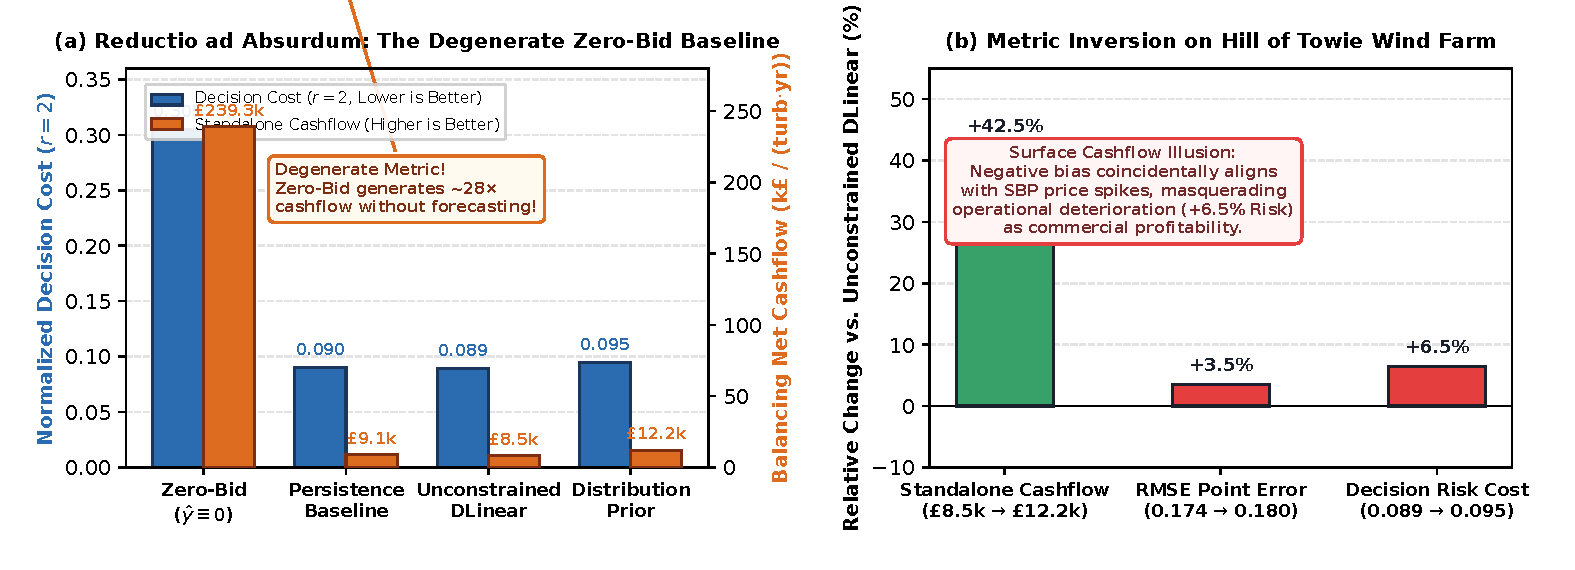
\includegraphics[width=\textwidth]{fig_market_decoupling.pdf}
\caption{Market Settlement Decoupling and Metric Inversion Diagnostic under Half-Hour Imbalance Accounting. (a) Reductio ad absurdum: the degenerate zero-bid settlement anomaly ($q \equiv 0$) incurs zero shortfall penalty and mechanically generates over \pounds 220k/turb$\cdot$yr in apparent cashflow without generating forecasts, exposing unhedged imbalance cashflow as an evaluation trap. (b) Empirical metric inversion on Hill of Towie, where distribution constraints increase nominal balancing cashflow by $+42.5\%$ while concurrently degrading genuine decision risk by $+6.5\%$ and RMSE by $+3.5\%$.}
\label{fig:market_decoupling}
\end{figure*}

Because $q \equiv 0 \le y_t$ holds almost surely for non-negative wind generation, the Zero-Bid strategy incurs exactly \textbf{\pounds 0.00 in shortfall penalties} across all three wind farms. In standalone unhedged balancing accounting, Zero-Bid mechanically generates massive apparent cashflows:
\begin{itemize}[leftmargin=*]
\item \textbf{Kelmarsh}: $+\pounds 223{,}882$/(turb$\cdot$yr);
\item \textbf{Hill of Towie}: $+\pounds 239{,}299$/(turb$\cdot$yr);
\item \textbf{Penmanshiel}: $+\pounds 243{,}450$/(turb$\cdot$yr).
\end{itemize}

We explicitly emphasize that \textbf{these six-figure sums represent uncontracted physical spill, not commercial profit or economic value}. In actual wholesale electricity markets (governed by the two-settlement identity $R_{\text{total}} = P_{\text{F}} \cdot q + P_{\text{imb}} \cdot (y - q)$ in Eq.~\eqref{eq:two_settlement}), bidding zero forfeits all forward contract revenue ($P_{\text{F}} \cdot q = 0$). When evaluated under the ground-truth asymmetric operational dispatch loss ($r=2, q=1/3$), Zero-Bid is heavily penalized, yielding normalized decision costs of $0.30409$ to $0.33689$ (matching the normalized mean capacity factor $\bar{y}$, Table~\ref{tab:zero_bid_diagnostic}).

Furthermore, on Hill of Towie, distribution regularization increases nominal balancing cashflow by $+42.5\%$ (\pounds 8,543 to \pounds 12,174/(turb$\cdot$yr); Table~\ref{tab:zero_bid_diagnostic}) while concurrently degrading normalized decision risk ($\text{Cost}_{\text{static}}$) by $+6.5\%$ and RMSE by $+3.5\%$ (Figure~\ref{fig:market_decoupling}b). This divergence occurs because the prior induces a systematic negative bias that happens to coincide with positive price spikes, creating apparent cashflow gains that mask operational dispatch degradation.

\subsection{Dynamic Market Settlement Diagnostic under 2017 UK BSC Prices}
To assess how physical constraints perform under non-stationary market conditions, we evaluated models across full-year 2017 UK Elexon BSC System Buy Prices in a stylized settlement diagnostic (Table~\ref{tab:paired_bootstrap}).

\begin{table*}[!t]
\centering
\vspace{-6pt}
\footnotesize
\renewcommand{\arraystretch}{0.80}
\setlength{\tabcolsep}{3.0pt}
\caption{7-Day Circular Block Paired Bootstrap Contrasts vs. Unconstrained DLinear under Calibrated Policy (2,000 Replications).}
\label{tab:paired_bootstrap}
\begin{threeparttable}
\begin{tabularx}{\textwidth}{p{2.2cm}p{3.2cm}>{\centering\arraybackslash}X>{\centering\arraybackslash}X>{\centering\arraybackslash}X}
\toprule
\textbf{Site} & \textbf{Method Contrast} & \textbf{Dynamic Cost Diff $\Delta \text{Cost}_{\text{dyn}}$} & \textbf{Shortfall Cashout Diff} & \textbf{Balancing Cashflow Diff} \\
 & & \textbf{(95\% CI)} & \textbf{\pounds/(turb$\cdot$yr) (95\% CI)} & \textbf{\pounds/(turb$\cdot$yr) (95\% CI)} \\
\midrule
\multirow{4}{=}{\textbf{Hill of Towie}} 
& Bounds vs.\ DLinear & $+0.000000$ ($[+0.000000, +0.000000]$) & $+\pounds 0.15$ ($[-0.17, +0.51]$) & $-\pounds 0.32$ ($[-1.37, +0.62]$) \\
& Power Curve vs.\ DLinear & $-0.000008$ ($[-0.000021, +0.000007]$) & $+\pounds 22.99$ ($[+10.93, +38.43]$) & $-\pounds 89.40$ ($[-133.51, -54.70]$) \\
& Distribution Prior vs.\ DLinear & \textbf{$+0.000766$ ($[+0.000277, +0.001201]$)} & \textbf{$-\pounds 578.57$ ($[-834.86, -367.51]$)} & \textbf{$+\pounds 1,481.27$ ($[+802.29, +2,203.32]$)} \\
& Ridge vs.\ DLinear & $-0.000733$ ($[-0.001315, -0.000125]$) & $+\pounds 192.50$ ($[-26.66, +445.74]$) & $-\pounds 1,151.96$ ($[-1,567.98, -795.28]$) \\
\midrule
\multirow{4}{=}{\textbf{Kelmarsh}} 
& Bounds vs.\ DLinear & $+0.000001$ ($[+0.000000, +0.000002]$) & $+\pounds 1.72$ ($[-0.01, +4.63]$) & $-\pounds 4.62$ ($[-12.67, +0.05]$) \\
& Power Curve vs.\ DLinear & $-0.000039$ ($[-0.000054, -0.000023]$) & $-\pounds 16.61$ ($[-33.12, +0.87]$) & $+\pounds 19.51$ ($[-27.76, +62.86]$) \\
& Distribution Prior vs.\ DLinear & \textbf{$+0.000932$ ($[+0.000423, +0.001385]$)} & \textbf{$+\pounds 932.56$ ($[+648.20, +1,236.74]$)} & \textbf{$-\pounds 3,264.86$ ($[-4,365.40, -2,223.50]$)} \\
& Ridge vs.\ DLinear & $+0.001338$ ($[+0.000917, +0.001794]$) & $+\pounds 750.61$ ($[+330.70, +1,151.06]$) & $-\pounds 690.94$ ($[-1,669.76, +409.51]$) \\
\bottomrule
\end{tabularx}
\begin{tablenotes}[flushleft]
\footnotesize
\item \textbf{Interpretation}: Negative shortfall cashout difference indicates cost reduction relative to unconstrained DLinear. Positive balancing cashflow difference indicates higher net cashflow component credited from the balancing mechanism. Confidence intervals estimated via 2,000 replications of 7-day circular block paired bootstrapping to account for temporal autocorrelation.
\end{tablenotes}
\end{threeparttable}
\end{table*}

Across dynamic settlement, physical constraints produce divergent operational outcomes across sites: on Kelmarsh, calibrated distribution constraints increase annual shortfall expenditure by \pounds 932.56/(turb$\cdot$yr) (95\% CI: $[+\pounds 648.20, +\pounds 1{,}236.74]$) and reduce net balancing cashflow by $-\pounds 3{,}264.86$/(turb$\cdot$yr). Conversely, on Hill of Towie, distribution constraints reduce annual shortfall expenditure by \pounds 578.57/(turb$\cdot$yr) and increase net balancing cashflow by \pounds 1{,}481.27/(turb$\cdot$yr) (95\% CI: $[+\pounds 802.29, +\pounds 2{,}203.32]$).

Methodologically, our framework strictly separates two orthogonal sources of empirical variation:
\begin{enumerate}[leftmargin=*]
\item \textbf{Temporal Autocorrelation Sampling Uncertainty (Delivery Period)}: The bootstrap intervals in Table~\ref{tab:paired_bootstrap} are estimated via 2,000 replications of 7-day circular block paired bootstrapping ($L=1{,}008$ steps), capturing atmospheric autocorrelation, weather regime shifts, and non-stationary price volatility.
\item \textbf{Initialization Stochasticity (Parameter Variance)}: The multi-seed dispersion metrics (mean $\pm$ standard deviation) in Table~\ref{tab:controlled_ablation} isolate parameter initialization randomness and mini-batch trajectories across identical training data.
\end{enumerate}

\subsection{Supporting Software Forensics: The Physics-Constrained Transformer}
Beyond evaluation metrics, establishing reliable empirical attribution requires verifying that executed software faithfully implements published mathematics. The Physics-Constrained Transformer (PCT \cite{pct2026}, \textit{Scientific Reports} 2026; commit \texttt{65941ec}) represents the sole publicly accessible training codebase for end-to-end physics-constrained Transformers and serves as an illustrative forensic case study.

In Section 2 of the PCT paper, the authors specify the symmetric Jensen--Shannon (JS) divergence:
\begin{equation}
\mathcal{L}_{\text{JS}}(P_{\text{pred}} \parallel P_{\text{ref}}) = \frac{1}{2} \text{KL}\left(P_{\text{pred}} \,\Big\|\, M\right) + \frac{1}{2} \text{KL}\left(P_{\text{ref}} \,\Big\|\, M\right),
\label{eq:js_divergence}
\end{equation}
where $M = \frac{1}{2}(P_{\text{pred}} + P_{\text{ref}})$.

However, static AST inspection of the official training script (\texttt{train\_clean.py}, lines 349--352) reveals that the computational graph evaluates:
\begin{equation}
\begin{split}
\mathcal{L}_{\text{code}} &= \frac{1}{2} \text{KL}\left(M \parallel P_{\text{pred}}\right) + \frac{1}{2} \text{KL}\left(M \parallel P_{\text{ref}}\right).
\end{split}
\label{eq:reverse_js}
\end{equation}
This occurs because PyTorch's \texttt{torch.nn.functional.kl\_div(input, target)} computes $\sum_i \text{target}_i (\log \text{target}_i - \text{input}_i) = \text{KL}(\text{target} \parallel \text{input})$. Passing \texttt{pred\_kde.log()} as input binds $P_{\text{pred}}$ to the denominator, executing what we designate the \textbf{reverse-argument JS form}.

Differentiating $\mathcal{L}_{\text{code}}$ directly with respect to $P_{\text{pred}, i}$ yields:
\begin{equation}
\frac{\partial \mathcal{L}_{\text{code}}}{\partial P_{\text{pred}, i}} = \frac{1}{4} \left[ \log \left(\frac{M_i^2}{P_{\text{pred}, i} P_{\text{ref}, i}}\right) + 1 - \frac{P_{\text{ref}, i}}{P_{\text{pred}, i}} \right].
\label{eq:reverse_js_gradient}
\end{equation}
Equation~\eqref{eq:reverse_js_gradient} exposes an analytical \textbf{inverse-density singularity}: whenever $P_{\text{pred}, i} \to 0$ in a region where empirical data exists ($P_{\text{ref}, i} > 0$), the ratio $\frac{P_{\text{ref}, i}}{P_{\text{pred}, i}}$ diverges as $\mathcal{O}(1/\epsilon)$. In contrast, for the mathematically specified Standard-JS in Eq.~\eqref{eq:js_divergence}, the partial derivative is bounded above by $\frac{1}{2}\ln 2 \approx 0.3466$ and exhibits only mild logarithmic divergence ($\mathcal{O}(|\log \epsilon|)$).

\begin{figure*}[!t]
\centering
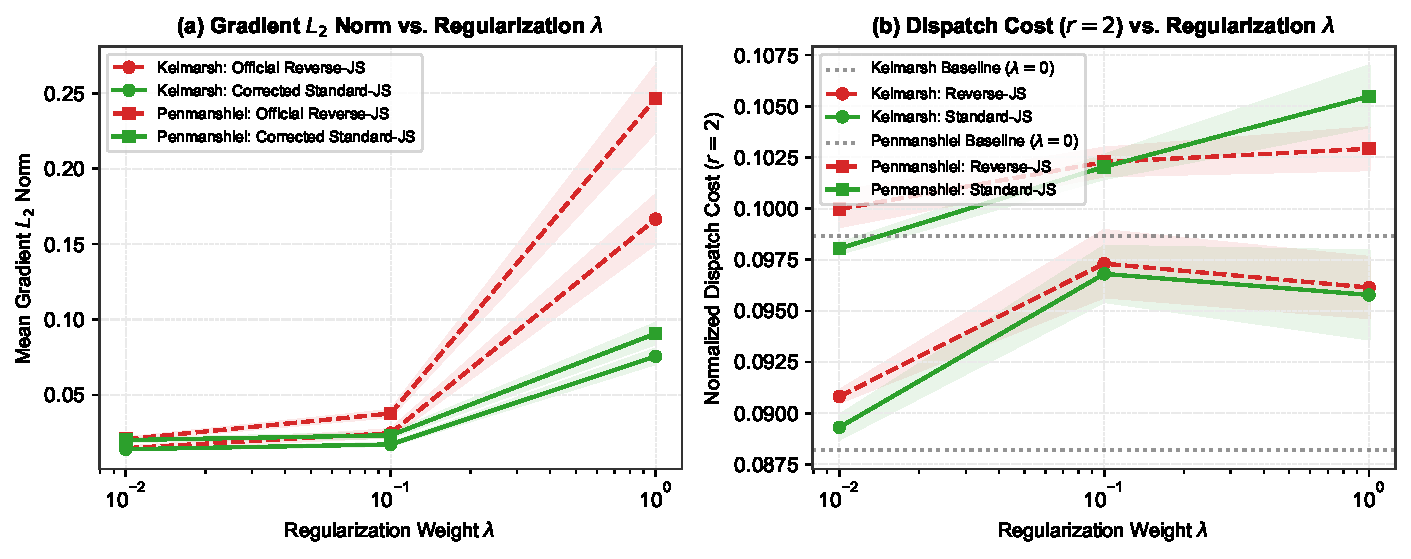
\includegraphics[width=\textwidth]{fig_pct_loss_empirical_contrast.pdf}
\caption{Empirical Optimization Contrast between Official Reverse-JS and Corrected Standard-JS on Kelmarsh and Penmanshiel. (a) Mean gradient $L_2$ norm: the reverse-argument JS form induces substantial gradient amplification at $\lambda = 1.0$ ($2.20\times$ on Kelmarsh, $2.72\times$ on Penmanshiel) due to the $-\frac{P_{\text{ref}, i}}{4 P_{\text{pred}, i}}$ singularity ($\mathcal{O}(1/\epsilon)$ in Eq.~\eqref{eq:reverse_js_gradient}). (b) Operational dispatch cost ($r=2$): Corrected Standard-JS prevents premature performance degradation at weak $\lambda=0.01$, while excessive regularization degrades dispatch across both distribution prior variants.}
\label{fig:pct_loss_empirical}
\end{figure*}

\paragraph{Empirical Gradient and Dispatch Contrast}
Empirical training on Kelmarsh and Penmanshiel across five seeds confirms that this implementation divergence materially alters optimization (Figure~\ref{fig:pct_loss_empirical}). At $\lambda = 1.0$, the reverse-argument JS form amplifies mean gradient $L_2$ norms by $2.20\times$ on Kelmarsh ($0.1665 \pm 0.0160$ vs.\ $0.0756 \pm 0.0048$) and by $2.72\times$ on Penmanshiel ($0.2465 \pm 0.0217$ vs.\ $0.0907 \pm 0.0067$; Figure~\ref{fig:pct_loss_empirical}a). At weak regularization ($\lambda = 0.01$ on Penmanshiel), Corrected Standard-JS achieves a dispatch cost of $0.09804 \pm 0.00024$, whereas the official reverse-argument implementation inflates dispatch cost to $0.09997 \pm 0.00086$ (a $+1.35\%$ degradation; Figure~\ref{fig:pct_loss_empirical}b). Under strong regularization ($\lambda = 1.0$), excessive penalization degrades operational dispatch across both distribution prior variants.

\paragraph{Negative Control: Algebraic Verification of 2D Product-Kernel KDE}
To establish an objective negative control and verify that our audit does not falsely report errors where none exist, we algebraically verified the tensor outer product $G = K_p^\top K_w \in \mathbb{R}^{B_p \times B_w}$ in the PCT codebase. Expanding the matrix product element at grid coordinate $(i,j)$ yields:
\begin{equation}
\left[ K_p^\top K_w \right]_{i,j} = \sum_{s=1}^N \phi\left( \frac{b_i^p - P_s}{h_p} \right) \cdot \phi\left( \frac{b_j^w - w_s}{h_w} \right).
\label{eq:kde_proof}
\end{equation}
Equation~\eqref{eq:kde_proof} is the exact analytical definition of a standard \textbf{paired 2D product-kernel Kernel Density Estimator} on correlated bivariate data. Because the summation contracts over concurrent sample index $s$, empirical joint coupling between wind speed and power is preserved. This confirms that software discrepancies in the audited codebase were strictly localized to the divergence argument order, rather than upstream kernel estimation.

\section{Discussion, Boundary Contracts, and Compliance Protocol}
\label{sec:discussion}

\subsection{Four Empirical Boundary Conditions for Physics-Constrained Models}
The scoping audit, algebraic code examination, and prospective ablations converge on four boundary conditions that determine when physical priors help, when they are neutral, and when they harm.

\paragraph{Sample Restriction and Prior Misspecification Vulnerability}
On Penmanshiel ($N_{\text{train}}=1,583$), the calibrated power curve prior at $\lambda=1.0$ reduces asymmetric dispatch cost from $0.09881 \pm 0.00027$ to $0.09760 \pm 0.00044$ ($-1.22\%$). A scale-matched scrambled pseudo-prior raises it to $0.16611 \pm 0.00335$ ($+68.1\%$). The divergence between these two outcomes---authentic priors securing modest downside protection while corrupted priors inflict severe operational damage---demonstrates a fundamental risk-return asymmetry: under strong regularization, whatever information the prior encodes is amplified, including its misspecifications. Cross-site comparisons cannot isolate this effect because they confound site topography with sample volume. In the data-rich regime (Kelmarsh, $N_{\text{train}}=5,098$), unconstrained DLinear ($0.08812$), genuine physics ($0.08791$), and scrambled prior ($0.08801$) are numerically clustered, indicating hypothesis-space saturation.

\paragraph{Low-Penalty Scale and Non-Specific Numerical Regularization}
At $\lambda = 0.01$ on Kelmarsh, a genuine physical prior ($0.08810 \pm 0.00009$) and a structurally scrambled pseudo-prior ($0.08801 \pm 0.00008$) yield closely matched decision costs with overlapping seed margins. When random power curve permutations reproduce the same outcome as domain aerodynamics, the penalty term behaves empirically as a non-specific regularizer / numerical smoothing term rather than encoding domain physical laws. Published claims of domain physical benefit under $\lambda \in [10^{-4}, 10^{-2}]$ require negative-control ablations and sensitivity testing at $\lambda \ge 0.1$ to be credible.

\paragraph{Monotonic Cost Inflation under Training Proxy Observation Staleness}
When physical constraint formulations rely on meteorological proxies to query empirical power curves during loss computation, practitioners may be tempted to substitute lagged historical observations when contemporaneous or forward weather forecasts are unavailable. Our lag scan ($k \in \{6, 12, 18, 36\}$ steps, 1\,h to 6\,h) demonstrates strictly monotonic cost inflation across all three wind farms. On Hill of Towie, dispatch risk climbs from $0.09022$ at $k=6$ to $0.09257$ at $k=36$, exceeding the unconstrained baseline ($0.08924$) at $k \approx 12$. We emphasize that this experiment characterizes the sensitivity of the training objective to temporal misalignment between the forecast horizon and the historical meteorological proxy, rather than an inference-time telemetry delay (the forecasting backbone takes only past power measurements during inference). Nonetheless, it demonstrates that offline regularization against lagged weather proxies rapidly erodes inductive guidance, presenting an operational limitation for proxy-dependent constraint designs.

\paragraph{Metric Decoupling and the Zero-Bid Diagnostic}
Under standard two-settlement market design, total generator revenue is $R_{\text{total}} = P_{\text{DA}} \cdot q + P_{\text{imb}} \cdot (y - q)$. Evaluations that drop the forward commitment term and report only balancing cashflow are measuring imbalance rent, not forecast skill. As an analytical imbalance-settlement and decision-risk diagnostic, the degenerate Zero-Bid baseline ($q \equiv 0$) provides a mathematical \textit{reductio ad absurdum}: it extracts £223k--£243k per turbine-year across all three farms without generating forecasts, simply by converting all physical generation into uncontracted spill rewarded at $P_{\text{imb}}$. This confirms that standalone unhedged balancing cashflows are decoupled from forecasting skill, and that assessing full commercial value requires joint modeling of forward contract revenue ($P_{\text{DA}} \cdot q$) and imbalance settlement. Operational evaluations must report asymmetric Pinball loss at the market penalty ratio or full two-settlement P\&L.

\subsection{External Validity Boundaries}
\label{sec:boundary_contract}
Five operational boundaries define the validity envelope of our empirical findings:

\paragraph{Boundary 1: Sample Volume and Hypothesis-Space Saturation}
Within-site learning curves confirm that physical constraint benefits concentrate under data-scarce regimes in our tested configurations ($N_{\text{train}} \le 1,000$, Figure~\ref{fig:within_site_learning_curve}). As training data expands to $N_{\text{train}} = 5{,}000$, hypothesis-space saturation reduces the gap between genuine-prior and unconstrained models to within 0.33\% on Kelmarsh, while scrambled priors remain severely detrimental throughout. Continuous corruption tests further establish a narrow fault-tolerance window ($\alpha^* \approx 0.07$ on Penmanshiel, Figure~\ref{fig:corruption_gradient}). Beyond this threshold, engineering drift exceeding 10\% aerodynamic capacity loss or $\pm 5\%$ anemometer bias flips the nominal physical prior from an asset into an operational liability.

\paragraph{Boundary 2: Proxy Misalignment and Observation Staleness}
For proxy-dependent physical constraints, regularization effectiveness depends on temporal alignment between meteorological proxies and target horizons ($k \le 6$ steps). Beyond this, monotonic cost inflation is observed on all three farms ($+2.6\%$ on Hill of Towie at $k=36$). Offline training objectives that substitute stale historical proxies for contemporaneous weather data induce substantial performance degradation.

\paragraph{Boundary 3: Market Clearing and Two-Settlement Structure}
Economic findings serve as an imbalance-settlement and decision-risk diagnostic bounded by two-settlement markets with asymmetric shortage penalties ($r \ge 1.0$) and UK BSC 30-minute discrete netting. Standalone imbalance cashflows do not represent full commercial value and do not generalize to symmetric single-settlement systems or flat feed-in tariffs.

\paragraph{Boundary 4: Computational Graph Audit and Implementation Parity}
Software conclusions apply to PCT commit \texttt{65941ec} and the computational graphs audited here. Unreleased proprietary codebases require independent static graph audit before implementation fidelity claims can be admitted.

\paragraph{Boundary 5: Literature Scoping Scope and Architectural Probe Envelopes}
The systematic literature audit is strictly bounded to the 46 studies identified under our PRISMA-ScR protocol; the documented 95.7\% code deficit and 50.0\% confounded ablation prevalence characterize reporting practices within this scoping cohort rather than an exhaustive census of all hybrid machine learning. Similarly, our PatchTST evaluations function as an architectural sensitivity probe under fixed nominal regularization ($\lambda=0.01$); while demonstrating that qualitative downside risk reduction persists across non-linear deep representations, joint cross-backbone $\lambda$ grid searches remain an open direction for future benchmarking.

\subsection{Two Conjectures Falsified During the Audit}
Two initial hypotheses were refuted during the empirical audit. First, forensic tensor derivation showed that PCT's product-kernel KDE preserves bivariate coupling algebraically, refuting the conjecture of marginal independence. Second, market diagnostic probing showed that post-calibration cashflow inversions are governed by settlement price asymmetries rather than physical regularizers. Documenting these falsification outcomes provides a transparent account of our investigative trajectory and prevents post-hoc rationalization.

\subsection{REFORMS-PCWPF Compliance Protocol}
\label{sec:reforms_pcwpf}
Table~\ref{tab:reforms_checklist} proposes five verification gates as a methodological reporting checklist for physics-constrained wind forecasting studies:

\begin{table*}[!t]
\centering
\footnotesize
\renewcommand{\arraystretch}{0.88}
\setlength{\tabcolsep}{3.5pt}
\caption{Methodological Verification Checklist for Physics-Constrained Wind Power Forecasting (Criteria C1--C5).}
\label{tab:verification_checklist}
\begin{threeparttable}
\begin{tabularx}{\textwidth}{p{1.4cm}p{2.6cm}>{\raggedright\arraybackslash}X>{\raggedright\arraybackslash}Xp{3.2cm}}
\toprule
\textbf{Criterion} & \textbf{Governance Dimension} & \textbf{Mandatory Audit Protocol} & \textbf{Common Pitfall / Anti-Pattern} & \textbf{Required Verification Artifact} \\
\midrule
\textbf{C1} & \textbf{Isolated Prior Ablation} & Train identical network backbones with constraint penalty $\lambda=0$ vs. $\lambda>0$ under identical seed schedules. & Confounding module excision (removing entire GNNs or attention blocks) with physical knowledge. & Table of $\lambda=0$ vs. $\lambda>0$ with identical parameter counts and multi-seed variances. \\
\midrule
\textbf{C2} & \textbf{Domain Specificity Control} & Evaluate pseudo-scrambled priors that preserve loss formulation, architecture, and regularization weight $\lambda$ while permuting physical relations. & Mistaking non-specific numerical regularization under weak penalty settings (e.g., $\lambda = 0.01$ under the present loss scaling) for domain reasoning. & Scrambled control performance curve and empirical specificity ratio ($p$-value contrast). \\
\midrule
\textbf{C3} & \textbf{Proxy Staleness Stress-Test} & If constraints depend on physical inputs (e.g., wind speed), scan historical proxy lag $k \in \{6, 12, 18, 36\}$ steps to evaluate proxy staleness when forward NWP forecasts are absent. & Assuming temporally aligned physical proxies when constructing the offline constraint target. & Observation staleness degradation curve demonstrating operational harm horizon. \\
\midrule
\textbf{C4} & \textbf{Metric Decoupling \& Accounting} & Report symmetric error (RMSE), non-negative asymmetric decision risk (Pinball), and test degenerate zero-bid anomaly baselines. & Reporting unhedged standalone imbalance cashflow in isolation, mistaking accidental price-spike alignment for skill. & Decoupled market evaluation coupling forward commitments and balancing cashflow. \\
\midrule
\textbf{C5} & \textbf{Computational Graph Parity} & Verify that software loss implementations match published mathematical equations in argument direction and normalization. & Argument order flip in asymmetric divergences (e.g., PyTorch \texttt{F.kl\_div}) causing reverse optimization. & Static code audit report and unit test verifying loss tensor gradient directions. \\
\bottomrule
\end{tabularx}
\begin{tablenotes}[flushleft]
\footnotesize
\item \textbf{Notes}: Derived from our empirical audit of 46 scoping studies and adapted from general machine-learning reporting principles \cite{kapoor2024reforms,walsh2021dome}. We propose C1--C5 as an operational reporting checklist for future physics-constrained renewable energy forecasting studies.
\end{tablenotes}
\end{threeparttable}
\end{table*}


\begin{itemize}
\item \textbf{Gate M1 (Parameter-Isolated Ablations):} Parameter-matched comparisons ($\lambda=0$ vs.\ $\lambda>0$) should be required to isolate physical prior contributions, avoiding submodule excisions (e.g., stripping GNN layers) that conflate representational capacity with domain knowledge.
\item \textbf{Gate M2 (Pseudo-Scrambled Negative Controls):} A minimum credible evaluation of physical reasoning claims should include scale-matched permutation controls to separate aerodynamic guidance from non-specific numerical smoothing.
\item \textbf{Gate M3 (Operational Proxy Staleness Stress-Tests):} Multi-step constraint evaluations should avoid assuming zero-latency future weather inputs, reporting performance across $k \in \{6, \dots, 36\}$ steps when forward NWP feeds are absent.
\item \textbf{Gate M4 (Coupled Two-Settlement Evaluation):} Evaluations should avoid standalone unhedged balancing cashflows, reporting instead asymmetric Pinball loss at the market penalty ratio or coupled two-settlement P\&L ($P_{\text{DA}} \cdot q + P_{\text{imb}} \cdot (y - q)$).
\item \textbf{Gate M5 (Static Computational Graph Audit):} Reviewers should expect executable training scripts or verified computational graphs, verifying that software loss execution matches published definitions in argument ordering and reduction semantics.
\end{itemize}

\section{Conclusion}
\label{sec:conclusion}

Three overarching conclusions emerge from this empirical audit regarding physics-constrained wind power forecasting.

First, at the literature and reporting level, studies in the audited scoping cohort reported exclusively within nominal operating envelopes (0/46 documenting failure regimes), while frequently relying on confounded module ablations and omitting public code. When computational graphs are subjected to static and gradient verification, implementations can diverge substantially from published equations. Establishing reliable scientific claims in physics-constrained machine learning requires open source code, computational graph verification, and form-matched negative controls.

Second, at the methodological and inductive level, physical priors function not as universal boosters, but as \textbf{conditional inductive guardrails}. In restricted training windows, authentic aerodynamic curves supply vital inductive regularization that curtails tail dispatch risk, exhibiting prior-specific mapping effects in this sample-restricted setting that cannot be attributed to data volume alone. As operational telemetry expands, purely data-driven models match or slightly exceed fixed priors---a dynamic interpreted through the lens of diminishing variance reduction and emerging structural approximation bias, though these mechanisms remain conceptual interpretations consistent with---not identified by---the observed learning curves. Furthermore, physical priors exhibit pronounced fragility under uncalibrated engineering drift and stale telemetry proxies (where decision risk exceeds the unconstrained reference by the first evaluated lag $k=6$ / 1\,h delay and deteriorates monotonically through $k=36$). Operational deployment therefore mandates adaptive regularization annealing and telemetry latency tolerance checks.

Third, at the operational decision level, symmetric regression metrics (RMSE and MAE) and standalone unhedged balancing cashflows structurally decouple from real-world dispatch risk. Symmetric metrics mask catastrophic tail under-predictions during shortfall events, while unhedged single-component settlement rewards degenerate, non-forecasting strategies. Forecasting models intended for grid integration must be optimized and audited against decision-aligned asymmetric dispatch objectives.

In conclusion, physics-constrained machine learning for energy systems must move beyond uncritical performance narratives. By institutionalizing form-matched negative controls, boundary stress tests, computational graph auditing, and decision-aligned evaluation (Criteria C1--C5), the field can transition toward verifiable, reproducible, and operationally dependable forecasting systems.


\appendix
\section{Mathematical Analysis of Decoupled Calibration Boundaries and Counterexamples}
\label{sec:appendix_proofs}

This appendix provides formal mathematical proofs for the two boundary counterexamples presented in Section~\ref{sec:theory}, delineating the theoretical limits of decoupled decision calibration.

\subsection{Counterexample 1: Constant Shift Invariance and Zero Excess Risk}
\label{subsec:counterexample1}

\begin{example}[Constant Shift Invariance]
\label{ex:constant_shift}
Let the target variable follow a uniform distribution $Y \sim U[0.25, 0.75]$, and consider an asymmetric cost ratio $r = 2$ ($\tau = 1/3$). Suppose an unconstrained model outputs the exact conditional expectation $f_0 = \mathbb{E}[Y] = 0.50$, while a physics-constrained model incurs a constant positive shrinkage shift $c = +0.05$, outputting $f_\lambda = 0.55$.
\end{example}

\paragraph{Prediction Representation Error (MSE)}
The mean squared prediction errors are:
\begin{align}
\text{MSE}(f_0) &= \text{Var}(Y) = \frac{0.50^2}{12} \approx 0.020833, \\
\text{MSE}(f_\lambda) &= \text{MSE}(f_0) + c^2 \approx 0.023333.
\end{align}
The physical constraint strictly inflates prediction MSE by $\Delta \text{MSE} = +0.0025$ ($+12.0\%$).

\paragraph{Uncalibrated Operational Dispatch Loss}
Under uncalibrated dispatch ($p = f$), the expected asymmetric loss is:
\begin{equation}
\begin{aligned}
\mathcal{R}_{\text{uncal}}(p) &= 2 \int_{0.25}^p (p - y) \cdot 2 \, dy + \int_p^{0.75} (y - p) \cdot 2 \, dy \\
&= 2(p - 0.25)^2 + (0.75 - p)^2.
\end{aligned}
\end{equation}
Evaluating at each prediction:
\begin{align}
\mathcal{R}_{\text{uncal}}(f_0 = 0.50) &= 2(0.25)^2 + (0.25)^2 = 0.187500, \\
\mathcal{R}_{\text{uncal}}(f_\lambda = 0.55) &= 2(0.30)^2 + (0.20)^2 = 0.220000.
\end{align}

\paragraph{Post-Hoc Decoupled Quantile Calibration}
The theoretical Bayes-optimal quantile at $\tau = 1/3$ is:
\begin{equation}
q_{1/3} = 0.25 + \tfrac{1}{3}(0.75 - 0.25) \approx 0.416667.
\end{equation}
Under decoupled quantile calibration, each model searches for its optimal scalar displacement:
\begin{align}
\delta_0^* &= q_{1/3} - f_0 \approx 0.416667 - 0.500000 = -0.083333, \\
\delta_\lambda^* &= q_{1/3} - f_\lambda \approx 0.416667 - 0.550000 = -0.133333.
\end{align}
Notice that the resulting dispatch commitments are identical:
\begin{equation}
p_0^* = f_0 + \delta_0^* = 0.416667, \quad p_\lambda^* = f_\lambda + \delta_\lambda^* = 0.416667.
\end{equation}
Consequently, the post-calibration operational risks are identical:
\begin{equation}
\mathcal{R}_{\text{cal}}(p_0^*) = \mathcal{R}_{\text{cal}}(p_\lambda^*) = 0.166667 \implies \Delta \mathcal{R}_{\text{disp}} \equiv 0.
\end{equation}

\paragraph{Theoretical Takeaway}
Counterexample 1 proves that \textbf{an increase in prediction MSE is compatible with invariant post-calibration operational risk}. When constraint-induced representation error consists of a uniform shift, scalar calibration absorbs the distortion entirely, establishing that strict positive excess risk lower bounds cannot hold unconditionally.

\subsection{Counterexample 2: Spatial Heteroscedasticity and Risk Reversal}
\label{subsec:counterexample2}

\begin{example}[Spatial Heteroscedasticity]
\label{ex:heteroscedasticity}
Let $X \in \{0, 1\}$ be a binary indicator with $P(X=0) = P(X=1) = 0.5$. Let the conditional target distributions exhibit heteroscedastic spread:
\begin{align}
Y \mid (X=0) &\sim U[0.20, 0.60] \quad (\mu_0 = 0.40, s_0 = 0.40), \\
Y \mid (X=1) &\sim U[0.30, 0.90] \quad (\mu_1 = 0.60, s_1 = 0.60).
\end{align}
Let the asymmetric cost ratio be $r = 2$ ($\tau = 1/3$). Consider two candidate forecasters: Model A (the unbiased conditional mean) with predictions $f_A(0) = 0.40$ and $f_A(1) = 0.60$; and Model B (a biased estimator with higher MSE) with predictions $f_B(0) = 0.40$ and $f_B(1) = 0.55$.
\end{example}

\paragraph{Prediction MSE Comparison}
The mean squared prediction errors are:
\begin{align}
\text{MSE}(f_A) &= 0.5 \left(\frac{0.40^2}{12}\right) + 0.5 \left(\frac{0.60^2}{12}\right) \nonumber \\
&= \frac{13}{600} \approx 0.021667, \\
\text{MSE}(f_B) &= \text{MSE}(f_A) + 0.5 (0.55 - 0.60)^2 \nonumber \\
&= 0.021667 + 0.001250 \approx 0.022917.
\end{align}
Model B has strictly higher prediction MSE by $\Delta \text{MSE} = +0.001250$ ($+5.8\%$).

\paragraph{Post-Hoc Global Scalar Calibration}
The local Bayes-optimal quantiles at $\tau = 1/3$ are:
\begin{align}
q_{1/3}(0) &= 0.20 + \tfrac{0.40}{3} = \tfrac{1}{3} \approx 0.333333, \\
q_{1/3}(1) &= 0.30 + \tfrac{0.60}{3} = 0.500000.
\end{align}
The Bayes-optimal operational dispatch loss is $\mathcal{R}(q_\tau) = 0.5(\frac{0.40}{3}) + 0.5(\frac{0.60}{3}) = \frac{1}{6} \approx 0.166667$. The local conditional densities are $f_0(y) = 2.5$ and $f_1(y) = 1.6667$.

Because local quantile-to-mean shifts differ ($\Delta_0 = q_{1/3}(0) - \mu_0 = -\frac{1}{15} \approx -0.066667$ versus $\Delta_1 = q_{1/3}(1) - \mu_1 = -0.100000$), a single global scalar offset $\delta^*$ cannot simultaneously achieve both local quantiles. The expected operational risk under global shift $\delta$ is:
\begin{equation}
\mathcal{R}(f + \delta) = 0.5 \, \mathcal{R}_0(f(0) + \delta) + 0.5 \, \mathcal{R}_1(f(1) + \delta).
\end{equation}

For \textbf{Model A} ($f_A = \mu$), the first-order optimality condition for $\delta_A^*$ is:
\begin{equation}
(r+1) \left[ 0.5 \cdot 2.5 (\delta_A^* - \Delta_0) + 0.5 \cdot 1.6667 (\delta_A^* - \Delta_1) \right] = 0,
\end{equation}
yielding the density-weighted optimal global offset:
\begin{align}
\delta_A^* &= \frac{2.5 (-\frac{1}{15}) + 1.6667 (-0.10)}{2.5 + 1.6667} \nonumber \\
&= \frac{-0.333333}{4.166667} = -0.080000.
\end{align}
The resulting excess operational risk for Model A is:
\begin{align}
&\mathcal{R}(f_A + \delta_A^*) - \mathcal{R}(q_\tau) \nonumber \\
&\quad = \frac{3}{2} \Big[ 1.25 (-0.080 + \tfrac{1}{15})^2 \nonumber \\
&\qquad\quad + 0.8333 (-0.080 + 0.100)^2 \Big] \nonumber \\
&\quad = \frac{15}{8} \left(-\frac{1}{75}\right)^2 + \frac{5}{4} \left(\frac{1}{50}\right)^2 \nonumber \\
&\quad = \frac{1}{3000} + \frac{1}{2000} = \frac{1}{1200} \approx 0.000833,
\end{align}
giving an absolute operational dispatch risk of:
\begin{equation}
\mathcal{R}_{\text{cal}}(f_A + \delta_A^*) = \frac{1}{6} + \frac{1}{1200} = \frac{201}{1200} = 0.167500.
\end{equation}

For \textbf{Model B} ($f_B(0) = 0.40, f_B(1) = 0.55$), the downward bias occurs on the higher-variance regime ($X=1$). The required local offsets become:
\begin{align}
\Delta_{0, B} &= q_{1/3}(0) - 0.40 = -\tfrac{1}{15} \approx -0.066667, \\
\Delta_{1, B} &= q_{1/3}(1) - 0.55 = 0.50 - 0.55 = -0.050000.
\end{align}
Notice that the discrepancy between regime offsets is halved: $|\Delta_{1, B} - \Delta_{0, B}| = \frac{1}{60} \approx 0.016667$, compared to $\frac{1}{30} \approx 0.033333$ for Model A. The optimal global offset for Model B is:
\begin{align}
\delta_B^* &= \frac{2.5 (-\frac{1}{15}) + 1.6667 (-0.050)}{2.5 + 1.6667} \nonumber \\
&= \frac{-0.166667 - 0.083333}{4.166667} = -0.060000.
\end{align}
The resulting excess operational risk for Model B is:
\begin{align}
&\mathcal{R}(f_B + \delta_B^*) - \mathcal{R}(q_\tau) \nonumber \\
&\quad = \frac{3}{2} \Big[ 1.25 (-0.060 + \tfrac{1}{15})^2 \nonumber \\
&\qquad\quad + 0.8333 (-0.060 + 0.050)^2 \Big] \nonumber \\
&\quad = \frac{15}{8} \left(\frac{1}{150}\right)^2 + \frac{5}{4} \left(-\frac{1}{100}\right)^2 \nonumber \\
&\quad = \frac{1}{12000} + \frac{1}{8000} = \frac{1}{4800} \approx 0.000208,
\end{align}
yielding an absolute operational dispatch risk of:
\begin{equation}
\mathcal{R}_{\text{cal}}(f_B + \delta_B^*) = \frac{1}{6} + \frac{1}{4800} = \frac{801}{4800} = 0.166875.
\end{equation}

Comparing the two post-calibration dispatch losses:
\begin{equation}
\mathcal{R}_{\text{cal}}(f_B + \delta_B^*) = 0.166875 < 0.167500 = \mathcal{R}_{\text{cal}}(f_A + \delta_A^*).
\end{equation}
Model B achieves a 75\% reduction in excess risk ($0.000208$ vs. $0.000833$) and strictly lower operational dispatch loss than the unbiased conditional mean, despite exhibiting $+5.8\%$ higher prediction MSE.

\paragraph{Theoretical Takeaway}
Counterexample 2 rigorously proves that \textbf{under conditional heteroscedasticity, a biased predictor with higher MSE can achieve strictly lower post-calibration dispatch loss than the true conditional mean}. This formalizes why the performance of physical constraints under decoupled calibration depends intricately on local error variance and environmental terrain.


\section*{Declaration of Interests}
The authors declare that they have no known competing financial interests or personal relationships that could have appeared to influence the work reported in this paper.

\section*{Author Contributions (CRediT)}
\textbf{Junyu Li}: Conceptualization, Methodology, Software, Formal analysis, Data curation, Investigation, Visualization, Project administration, Writing -- original draft, Writing -- review \& editing. \textbf{Juntao Du}: Methodology (review protocol), Validation, Data curation (scoping extraction double-coding), Writing -- review \& editing.

\section*{Declaration of Generative AI in the Writing Process}
During the preparation of this work, the authors used ChatGPT and Google Gemini to assist with literature synthesis, manuscript organization, language refinement, code review, and consistency checking. All scientific claims, calculations, references, experimental results, and final wording were independently reviewed and verified by the authors, who take full responsibility for the content.

\section*{Acknowledgments}
We thank the open science teams at Zenodo, Cubico Sustainable Investments, RES, TRIG, and Elexon for maintaining transparent public repositories of operational renewable energy telemetry and market clearing records. Computations were supported by dedicated high-performance computing infrastructure.

\section*{Data and Code Availability}
Raw operational SCADA telemetry from the Kelmarsh (DOIs: \href{https://doi.org/10.5281/zenodo.5841834}{10.5281/zenodo.5841834}) and Penmanshiel (\href{https://doi.org/10.5281/zenodo.5946808}{10.5281/zenodo.5946808}) wind farms is openly available on Zenodo under CC-BY 4.0 licenses from Cubico Sustainable Investments. Operational SCADA telemetry from the Hill of Towie wind farm is openly available on Zenodo under CC-BY 4.0 license released by RES on behalf of The Renewables Infrastructure Group (TRIG) (DOI: \href{https://doi.org/10.5281/zenodo.20204946}{10.5281/zenodo.20204946}). Elexon System Buy Price records are freely accessible through the Elexon BMRS portal under the UK Open Government Licence v3.0. The complete code suite, AST auditing scripts, and the 46-study scoping extraction database with verbatim quotes and multi-coder consensus scores are openly accessible for peer review via the anonymous repository: \url{https://github.com/anonymous-audit/pcwpf-audit}.

\setlength{\bibsep}{2.5pt plus 0.5pt minus 0.5pt}
\small
\bibliography{refs}

\end{document}
